% Options for packages loaded elsewhere
\PassOptionsToPackage{unicode,citecolor=black}{hyperref}
\PassOptionsToPackage{hyphens}{url}
\PassOptionsToPackage{dvipsnames,svgnames,x11names}{xcolor}
%
\documentclass[
  authoryear,
  preprint,
  3p,
  onecolumn]{elsarticle}

\usepackage{amsmath,amssymb}
\usepackage{iftex}
\ifPDFTeX
  \usepackage[T1]{fontenc}
  \usepackage[utf8]{inputenc}
  \usepackage{textcomp} % provide euro and other symbols
\else % if luatex or xetex
  \usepackage{unicode-math}
  \defaultfontfeatures{Scale=MatchLowercase}
  \defaultfontfeatures[\rmfamily]{Ligatures=TeX,Scale=1}
\fi
\usepackage{lmodern}
\ifPDFTeX\else  
    % xetex/luatex font selection
\fi
% Use upquote if available, for straight quotes in verbatim environments
\IfFileExists{upquote.sty}{\usepackage{upquote}}{}
\IfFileExists{microtype.sty}{% use microtype if available
  \usepackage[]{microtype}
  \UseMicrotypeSet[protrusion]{basicmath} % disable protrusion for tt fonts
}{}
\makeatletter
\@ifundefined{KOMAClassName}{% if non-KOMA class
  \IfFileExists{parskip.sty}{%
    \usepackage{parskip}
  }{% else
    \setlength{\parindent}{0pt}
    \setlength{\parskip}{6pt plus 2pt minus 1pt}}
}{% if KOMA class
  \KOMAoptions{parskip=half}}
\makeatother
\usepackage{xcolor}
\setlength{\emergencystretch}{3em} % prevent overfull lines
\setcounter{secnumdepth}{5}
% Make \paragraph and \subparagraph free-standing
\ifx\paragraph\undefined\else
  \let\oldparagraph\paragraph
  \renewcommand{\paragraph}[1]{\oldparagraph{#1}\mbox{}}
\fi
\ifx\subparagraph\undefined\else
  \let\oldsubparagraph\subparagraph
  \renewcommand{\subparagraph}[1]{\oldsubparagraph{#1}\mbox{}}
\fi


\providecommand{\tightlist}{%
  \setlength{\itemsep}{0pt}\setlength{\parskip}{0pt}}\usepackage{longtable,booktabs,array}
\usepackage{calc} % for calculating minipage widths
% Correct order of tables after \paragraph or \subparagraph
\usepackage{etoolbox}
\makeatletter
\patchcmd\longtable{\par}{\if@noskipsec\mbox{}\fi\par}{}{}
\makeatother
% Allow footnotes in longtable head/foot
\IfFileExists{footnotehyper.sty}{\usepackage{footnotehyper}}{\usepackage{footnote}}
\makesavenoteenv{longtable}
\usepackage{graphicx}
\makeatletter
\def\maxwidth{\ifdim\Gin@nat@width>\linewidth\linewidth\else\Gin@nat@width\fi}
\def\maxheight{\ifdim\Gin@nat@height>\textheight\textheight\else\Gin@nat@height\fi}
\makeatother
% Scale images if necessary, so that they will not overflow the page
% margins by default, and it is still possible to overwrite the defaults
% using explicit options in \includegraphics[width, height, ...]{}
\setkeys{Gin}{width=\maxwidth,height=\maxheight,keepaspectratio}
% Set default figure placement to htbp
\makeatletter
\def\fps@figure{htbp}
\makeatother

\usepackage{gensymb}
\usepackage{nth}
\usepackage{booktabs}
\makeatletter
\@ifpackageloaded{caption}{}{\usepackage{caption}}
\AtBeginDocument{%
\ifdefined\contentsname
  \renewcommand*\contentsname{Table of contents}
\else
  \newcommand\contentsname{Table of contents}
\fi
\ifdefined\listfigurename
  \renewcommand*\listfigurename{List of Figures}
\else
  \newcommand\listfigurename{List of Figures}
\fi
\ifdefined\listtablename
  \renewcommand*\listtablename{List of Tables}
\else
  \newcommand\listtablename{List of Tables}
\fi
\ifdefined\figurename
  \renewcommand*\figurename{Figure}
\else
  \newcommand\figurename{Figure}
\fi
\ifdefined\tablename
  \renewcommand*\tablename{Table}
\else
  \newcommand\tablename{Table}
\fi
}
\@ifpackageloaded{float}{}{\usepackage{float}}
\floatstyle{ruled}
\@ifundefined{c@chapter}{\newfloat{codelisting}{h}{lop}}{\newfloat{codelisting}{h}{lop}[chapter]}
\floatname{codelisting}{Listing}
\newcommand*\listoflistings{\listof{codelisting}{List of Listings}}
\makeatother
\makeatletter
\makeatother
\makeatletter
\@ifpackageloaded{caption}{}{\usepackage{caption}}
\@ifpackageloaded{subcaption}{}{\usepackage{subcaption}}
\makeatother
\makeatletter
\@ifpackageloaded{sidenotes}{}{\usepackage{sidenotes}}
\@ifpackageloaded{marginnote}{}{\usepackage{marginnote}}
\makeatother
\journal{J. Acoust. Soc. Am.}
\ifLuaTeX
  \usepackage{selnolig}  % disable illegal ligatures
\fi
\usepackage[]{natbib}
\bibliographystyle{elsarticle-harv}
\IfFileExists{bookmark.sty}{\usepackage{bookmark}}{\usepackage{hyperref}}
\IfFileExists{xurl.sty}{\usepackage{xurl}}{} % add URL line breaks if available
\urlstyle{same} % disable monospaced font for URLs
\hypersetup{
  pdftitle={Investigating urban soundscapes of the COVID-19 lockdown: A predictive soundscape modeling approach},
  pdfauthor={Andrew Mitchell; Tin Oberman; Francesco Aletta; Magdalena Kachlicka; Matteo Lionello; Mercede Erfanian; Jian Kang},
  pdfkeywords={Soundscape, Psychological acoustics, Acoustic
modeling, Acoustic noise, Acoustic ecology, Signal processing, Urban
development, Regression analysis},
  colorlinks=true,
  linkcolor={blue},
  filecolor={Maroon},
  citecolor={Blue},
  urlcolor={Blue},
  pdfcreator={LaTeX via pandoc}}

\setlength{\parindent}{6pt}
\begin{document}

\begin{frontmatter}
\title{Investigating urban soundscapes of the COVID-19 lockdown: A
predictive soundscape modeling approach}
\author[1]{Andrew Mitchell%
\corref{cor1}%
}
 \ead{andrew.mitchell.18@ucl.ac.uk} 
\author[1]{Tin Oberman%
%
}
 \ead{t.oberman@ucl.ac.uk} 
\author[1]{Francesco Aletta%
%
}
 \ead{f.aletta@ucl.ac.uk} 
\author[1]{Magdalena Kachlicka%
%
}

\author[1]{Matteo Lionello%
%
}

\author[1]{Mercede Erfanian%
%
}

\author[1]{Jian Kang%
%
}
 \ead{j.kang@ucl.ac.uk} 

\affiliation[1]{organization={University College London, Institute for
Environmental Design and Engineering},addressline={Central House, 14
Upper Woburn Place},city={London},postcode={WC1H 0NN},postcodesep={}}

\cortext[cor1]{Corresponding author}







        
\begin{abstract}
The unprecedented lockdowns due to COVID-19 in spring 2020 triggered
changes in human activities in public spaces. A predictive modeling
approach was developed to characterize the changes in the perception of
the sound environment when people could not be surveyed. Building on a
database of soundscape questionnaires (\(N=1,136\)) and binaural
recordings (\(N=687\)) collected in 13 locations across London and
Venice during 2019, new recordings (\(N=571\)) were made in the same
locations during the 2020 lockdowns. Using these 30-second-long
recordings, linear multi-level models were developed to predict
soundscape pleasantness (\(R^2=0.85\)) and eventfulness (\(R^2=0.715\))
during the lockdown and compare changes for each location. Performance
was above average for comparable models. An online listening study also
investigated the change in sound sources within the spaces. Results
indicate: 1) human sounds were less dominant and natural sounds more
dominant across all locations; 2) contextual information is important
for predicting pleasantness but not for eventfulness; 3) perception
shifted towards less eventful soundscapes and to more pleasant
soundscapes for previously traffic-dominated locations, but not for
human- and natural-dominated locations. This study demonstrates the
usefulness of predictive modeling and the importance of considering
contextual information when discussing the impact of sound level
reductions on the soundscape.
\end{abstract}





\begin{keyword}
    Soundscape \sep Psychological acoustics \sep Acoustic
modeling \sep Acoustic noise \sep Acoustic ecology \sep Signal
processing \sep Urban development \sep 
    Regression analysis
\end{keyword}
\end{frontmatter}
    \section{Introduction}\label{sec-intro}

The global emergency caused by the COVID-19 pandemic in early 2020
required national lockdown measures across the world, primarily
targeting human activity. In the United Kingdom, construction and
transport were allowed to continue, but a decrease in activity was
observed \citep{Hadjidemetriou2020impact}. In other countries, such as
Italy, the restrictions were more severe and even included limiting
people's movement to a certain radius from their place of residence
\citep{Ren2020Pandemic}. The explorations in environmental acoustics of
lockdown conditions across the world have revealed various degrees of
impact on the acoustic environment, with researchers reporting
reductions in noise levels affecting the population at the scale of
urban agglomerations such as Ruhr Area in Germany
\citep{Hornberg2021Impact} and conurbations in the south of France
\citep{Munoz2020Lockdown}. Impacts have also been reported at a scale of
a multimillion city such as Madrid \citep{Asensio2020Changes} or
Barcelona \citep{BonetSola2021Soundscape} as well as at a more local,
city-center or even public space-scale in cities such as Stockholm
\citep{Rumpler2021Noise}, London \citep{Aletta2020Assessing}, Girona
\citep{AlsinaPages2021Changes}, or Granada \citep{VidaManzano2021sound}.
In general, these studies have demonstrated a decrease in urban noise
levels and indicated a difference in the amount the level decreased
depending on the type of space investigated (e.g.~parks, urban squares,
etc.) and the type of human activity characteristic for the space, with
higher reductions in places typically associated with human sounds and
activities such as shopping and tourism.

Those studies were mostly focused around the \(L_{Aeq}\), as well as a
standardization approach to reporting subsequent changes in soundscape
proposed by \citet{Asensio2020Taxonomy}. They were not able to reveal
the perceptual impact of such conditions in public spaces also because
of: 1) the lack of subjective data for the exact or comparable locations
in previous years; and 2) the lack of participants present in public
spaces during the lockdown, hence the inability to collect soundscape
data in situ. \citet{Munoz2020Lockdown} combined noise measurements with
an online questionnaire deployed to residents, some of which were
residing in the areas covered by the noise monitoring network available.
The participants were asked to recall how their lockdown area sounded
before and during the first lockdown in 2020 and to describe the
perceived change. They observed a consistent reduction in levels,
followed by the perceived reduction of transport sounds (air and road)
and an increase of natural sounds, while the resulting environment was
described as pleasant, calm, and peaceful. By combining field recordings
and focus groups, \citet{Sakagami2020How} and
\citet{Lenzi2021Soundscape} observed changes in the sound source
composition and the affective quality of soundscape in a residential
area in Kobe, Japan and a public space in Getxa, Spain, respectively,
during the different stages of the lockdown period. Following the easing
of lockdown measures, a decrease in animal and traffic sounds was
observed in Kobe, while an increase in eventfulness, loudness, and
presence of human sound sources, followed by a decrease in pleasantness,
was shown in Getxa.

\citet{Aletta2020Assessing} explored the impacts of the COVID-19
lockdowns on the acoustic environment in London in particular, through
many short-term (30s) binaural recordings. This study revealed that
average reductions in the various locations considered ranged from 10.7
dB (\(L_{Aeq}\)) to 1.2 dB, with an overall average reduction of 5.4 dB.
This metric-reporting focused approach left the following research
questions unanswered: how would people have perceived these spaces as a
result of this change in acoustic environment (RQ1), and would these
sound level reductions result in improvements to the soundscape of the
spaces (RQ2)? The 1st research question (RQ1), addressing the perceptual
effect of the change in urban soundscape induced by the lockdowns, can
be further broken down into the following questions: how was the sound
source composition influenced by the change; how would the affective
response to the acoustic environment in lockdowns change; and could this
demonstrate the effect of human activities on the perception of an
acoustic environment in general?

These questions arise out of the soundscape approach, which is
characterized by prioritizing the perceptual effect of an acoustic
environment by taking into account the interaction of sound sources,
context, and the person perceiving it
\citep{ISO12913Part1, Truax1999Handbook}, bringing together objective
and subjective factors. The soundscape approach to noise mitigation and
management is being recognized as a response to arising environmental
requirements on noise pollution and sustainability, such as the
regulation of quiet areas in Europe
\citep{EuropeanUnion2002Directive, Kang2018Impact, Radicchi2021Sound}.
This has been further formalized in \citet{ISO12913Part2} via the
adoption of the circumplex model of soundscape
\citep{Axelsson2010principal}, in which the perception of a soundscape
can be described in terms of its pleasantness and eventfulness, as one
of the standard methods of soundscape assessment.

Soundscape research is therefore traditionally rooted in environmental
acoustics and environmental psychology, typically dealing with outdoor
spaces \citep{Torresin2020Indoor} and urban open spaces, where parks and
squares are often used as case study sites \citep{Kang2006Urban}. A
soundscape assessment typically requires people to be surveyed but the
presence of people at a location influences assessment
\citep{Aletta2018Towards} and `quiet places' usually require low numbers
of users to remain quiet, which limits the possibility of an assessment.
Even in a crowded public space, soundscape surveys are demanding as they
require significant resources to carry out at scale, limiting their
widespread application \citep{Mitchell2020Soundscape}. Therefore, a need
for a predictive model arises to overcome this limitation and improve
the implementation of the soundscape approach into everyday planning and
management practices.

According to a recent review of predictive soundscape models from
\citet{Lionello2020systematic}, the degree of employing auditory and
non-auditory factors in soundscape prediction varies with some studies
relying on contextual, personal/demographic
\citep{Erfanian2021Psychological, Tarlao2020Investigating} or social
media \citep{Aiello2016Chatty} data entirely to predict and generate
soundscape features. Some methods also incorporate perceptually-derived
features, such as subjective sound level and visual pleasantness as
predictors \citep{Lionello2020systematic}. In general, these methods
which incorporate perceptually-derived inputs achieve better accuracy
rates than those which don't, however this perception information must
also be obtained from people via a survey and therefore are unsuitable
for predictive modeling where surveys are not possible. For example,
\citet{Ricciardi2015Sound} proposed two models based on data collected
from a smartphone application to predict urban sound quality indicators
based on linear regressions. The first model which incorporated
perceptually-derived input features (visual quality and familiarity)
achieved an \(R^2\) of 0.72, while a second model without these features
achieved an \(R^2\) of 0.58. This indicates the necessity for
considering and accounting for the influence which contextual factors in
a space have on the relationship between the sound environment itself
and the listener's perception of it (i.e.~the soundscape) while also
highlighting the challenges associated with a predictive model which
depends only on measurable features.

Therefore, a third research question arises: what are the key features
needed for a soundscape prediction model based on comprehensive acoustic
on-site measurements to be used for assessing locations with low social
presence or in situations where conducting surveys is impractical (RQ3)?

\section{Materials and methods}\label{materials-and-methods}

This study was conducted via initial onsite data collection campaigns in
Central London and Venice in 2019 before the outbreak of COVID-19 as
part of the Soundscape Indices (SSID) project
\citep{Mitchell2020Soundscape} and in 2020 during the strictest part of
the lockdowns \citep{Aletta2020Assessing}, including objective acoustic
data (2019 and 2020) and subjective responses (2019 only). The full in
situ dataset, as described in this section, has been made publicly
available as `The International Soundscape Database (V0.2.1)' on
Zenodo\footnote{See \url{https://zenodo.org/record/5654747} for ``The
  International Soundscape Database (V0.2.1)'' (Last viewed 11/9/21)}\citep{Mitchell2021International}.

Using both 2019 and 2020 binaural recordings, an online listening
experiment was conducted to provide an understanding about the change in
sound source composition. The 2019 onsite questionnaire data were used
to define the dominant sound source at each location as a starting point
for interpreting soundscape change. A predictive model was developed to
reveal the change in the perceived pleasantness and eventfulness using
objective acoustic data and location to predict subjective responses.
Although the initial (2019) dataset contains additional locations
(specifically, in Spain, the Netherlands, and China), due to the nature
of this study as a reaction to the strict movement and activity
restrictions, the sites which could be included in the lockdown (2020)
measurement campaigns were limited to locations where staff and
equipment had access and where recordings could be undertaken during the
spring of 2020.

The sites were selected to provide a mixture of sizes and uses, varying
in typology ranging from paved squares to small and large parks to
waterside spaces across both cities. Throughout the text they are
indexed via a LocationID based on the location's name (e.g.~CamdenTown,
SanMarco), while a more in-depth overview of each is given in
supplementary material\footnote{See supplementary material at
  \url{https://www.scitation.org/doi/suppl/10.1121/10.0008928} for site
  descriptions per ISO/TS (2018) featuring the address, overall
  psychoacoustic characteristics of the location, typical use of each
  location, and pictures taken during the survey sessions.}. London is
taken as an example of a large, typically noisy city while the Venice
sample provides a unique look at spaces with typically very high human
activity levels and no road traffic activity. In particular, the 2019
Venice surveys were taken to coincide with the yearly Carnevale festival
in order to capture its distinct soundscape.

The ISO/TS 12913 \citep{ISO12913Part2} series were consulted for
reporting on soundscape data. A detailed description of the 2019 survey
campaigns is featured throughout the paper and in the public database.
This study was approved by departmental UCL IEDE Ethics Committee on
17th July 2018 for onsite data collection and on the 2nd of June 2020
for the on-line listening experiment and is conducted in adherence to
the ethical requirements of the Declaration of Helsinki
\citep{WMA2013World}.

\subsection{Onsite data: Questionnaires, binaural measurements, and
recordings}\label{onsite-data-questionnaires-binaural-measurements-and-recordings}

The initial onsite data collection featured both questionnaire data
collected from the general public and acoustic measurements, conducted
across thirteen urban locations (in London \(N=11\), in Venice \(N=2\))
between the 28th of February and the 21st of June 2019, with additional
sessions in July and October 2019. Although the total survey period in
2019 extended over several seasons, the surveys at any individual
location did not extend over seasons with different occupancy patterns.
A total of 1,318 questionnaire responses were collected from the general
population across the measurement points during 1 -- 3 hour-long
campaigns in both cities in 2019, accompanied by 693 approximately
30-second long 24-bit 44.1 kHz binaural recordings. After data cleaning,
each of the 13 locations was characterized by between 14 to 80
recordings and between 24 to 147 questionnaire responses. Mean age of
the participants was 33.8, with a standard deviation of 14.57 (45\%
male, 53.8\% female, 0.4\% non-conforming, 0.9\% prefer-not-to-say).

Although recent results from both \citet{Tarlao2020Investigating} and
\citet{Erfanian2021Psychological} indicate the important influence of
personal and demographic factors -- in particular age and gender -- on
soundscape perception, these factors were not included as potential
features in the modeling process. Given the nature of this study as
addressing a scenario when people could not be surveyed, no additional
demographic information is available in the lockdown case to be fed into
the model and is therefore not useful to include for the development and
application of this specific predictive model. This information is
reported throughout the study simply to provide further context to the
data collection.

The subsequent measurement campaign in 2020 mimicked the binaural
recording strategy applied in the initial campaign and was performed
between the \nth{6} and the 25th of April 2020 in both cities, this time
excluding the questionnaire. An additional 571 binaural recordings were
collected on-site in 2020.

\subsubsection{Data collection}\label{data-collection}

The 2019 data collection was performed across all the locations using
the protocol based on the Method A of the \citet{ISO12913Part2}, as
described in \citet{Aletta2020Assessing} and
\citet{Mitchell2020Soundscape}, collected either via handheld tablets or
paper copies of the questionnaire. The full questionnaire and data
collection procedure are given in \citet{Mitchell2020Soundscape},
however the key parts used for this study are those addressing sound
source dominance and perceived affective quality (PAQ).

Participants are first asked to rate the perceived dominance of several
sound sources, as assessed via a 5-point Likert scale, coded from 1 (Not
at all) to 5 (Dominates completely). The sound sources are split into
four categories: Traffic noise, Other noise, Human sounds, and Natural
sounds and each is rated separately. Next are the 8 PAQs which make up
the circumplex model of soundscape \citep{Axelsson2010principal}:
pleasant, chaotic, vibrant, uneventful, calm, annoying, eventful, and
monotonous. These are assessed on a 5-point Likert scale from 1
(Strongly disagree) to 5 (Strongly agree). In order to simplify the
results and allow for modeling the responses as continuous values, the 8
PAQs undergo a trigonometric projection to reduce them onto the two
primary dimensions of pleasant and eventful, according to the procedure
outlined in Part 3 of the ISO 12913 series \citep{ISO12913Part3}. In
order to distinguish the projected values from the Likert-scale PAQ
responses, the projected values will be referred to as ISOPleasant and
ISOEventful and can be considered to form an x-y coordinate point (x =
ISOPleasant, y = ISOEventful) as explained in detail in
\citet{Lionello2021Introducing}.

The calibrated binaural device SQobold with BHS II by Head Acoustics was
used in both campaigns at all the locations by various operators to
capture acoustic data, as mentioned in the acknowledgments. Following
the established onsite protocol \citep{Mitchell2020Soundscape}, when
participants were stopped in a group and filled in their responses
simultaneously, a single binaural recording was used to capture their
experience as a group. The purpose behind this sampling strategy was to
obtain data from the perspective of a typical user, corresponding to a
range of individual experiences available within an urban open space.
These recordings are indexed by a GroupID such that the recording for
each group is matched up to each of the corresponding respondents and
their individual survey responses.

\subsubsection{Data cleaning}\label{data-cleaning}

The cleaning of the samples was conducted using the ArtemiS SUITE 11.
The researcher discarded or cropped whole recordings, or its parts
affected by wind gusts or containing noises and speech generated by the
recording operator by accident or for the purpose of explaining the
questionnaire to a participant. This resulted in 1,258 binaural
recordings then processed further, as described in
Section~\ref{sec-psychoacousticAnalysis}. Psychoacoustic analyses are
shown in the publicly available database\footnote{See
  \url{https://zenodo.org/record/5654747} for ``The International
  Soundscape Database (V0.2.1)'' (Last viewed 11/9/21)}.

In order to maintain data quality and exclude cases where respondents
either clearly did not understand the PAQ adjectives or intentionally
misrepresented their answers, surveys for which the same response was
given for every PAQ (e.g.~`Strongly agree' to all 8 attributes) were
excluded prior to calculating the ISO projected values. This is
justified as no reasonable respondent who understood the questions would
answer that they `strongly agree' that a soundscape is pleasant and
annoying, calm and chaotic, etc. Cases where respondents answered
`Neutral' to all PAQs are not excluded in this way, as a neutral
response to all attributes is not necessarily contradictory. In
addition, surveys were discarded as incomplete if more than 50\% of the
PAQ and sound source questions were not completed.

The site characterization per \citet{ISO12913Part2} is available in the
supplementary material\footnote{See supplementary material at
  \url{https://www.scitation.org/doi/suppl/10.1121/10.0008928} for site
  descriptions per ISO/TS (2018) featuring the address, overall
  psychoacoustic characteristics of the location, typical use of each
  location, and pictures taken during the survey sessions.} and public
database\footnote{See \url{https://zenodo.org/record/5654747} for ``The
  International Soundscape Database (V0.2.1)'' (Last viewed 11/9/21)},
featuring the address, overall psychoacoustic characteristics of the
location, typical use of each location, and pictures taken during the
survey sessions.

\subsubsection{Psychoacoustic
analyses}\label{sec-psychoacousticAnalysis}

The binaural recordings were analyzed in ArtemiS SUITE 11 to calculate
the suite of 11 acoustic and psychoacoustic features given in
Table~\ref{tbl-psychoacoustics} to be used as initial predictors. The
(psycho)acoustic predictors investigated were selected in order to
describe many aspects of the recorded sound -- in particular, the goal
was to move beyond a focus on sound level, which currently dominates the
existing literature on the acoustic effects of lockdowns noted in
Section~\ref{sec-intro}. In all, they are expected to reflect the sound
level (\(L_{Aeq}\)), perceived sound level (Loudness), spectral content
(Sharpness, \(L_{Ceq}-L_{Aeq}\), Tonality), temporal character or
predictability (Impulsiveness, Fluctuation Strength, Relative Approach),
and overall annoyance (Psychoacoustic Annoyance). These metrics have
been proposed as indicators to predict perceptual constructs of the
soundscape \citep{Aletta2016Soundscape, Aletta2017Dimensions} and have
shown promise when combined together to form a more comprehensive model
applied to real-world sounds \citep{Orga2021Multilevel}. The maximum
value from the left and right channels of the binaural recording are
used, as suggested in \citet{ISO12913Part3}.

\begin{longtable}[]{@{}
  >{\raggedright\arraybackslash}p{(\columnwidth - 6\tabcolsep) * \real{0.3176}}
  >{\centering\arraybackslash}p{(\columnwidth - 6\tabcolsep) * \real{0.2235}}
  >{\centering\arraybackslash}p{(\columnwidth - 6\tabcolsep) * \real{0.1176}}
  >{\raggedright\arraybackslash}p{(\columnwidth - 6\tabcolsep) * \real{0.3412}}@{}}
\caption{Psychoacoustic features considered for inclusion in the
predictive models. All metrics are calculated for the full length of the
recording (\(\sim30s\)). As recommended by \citet{ISO2017Acoustics} and
\citet{ISO12913Part2}, the 5th percentile of Loudness is used rather
than the average.}\label{tbl-psychoacoustics}\tabularnewline
\toprule\noalign{}
\begin{minipage}[b]{\linewidth}\raggedright
\textbf{Feature}
\end{minipage} & \begin{minipage}[b]{\linewidth}\centering
\textbf{Symbol}
\end{minipage} & \begin{minipage}[b]{\linewidth}\centering
\textbf{Unit}
\end{minipage} & \begin{minipage}[b]{\linewidth}\raggedright
\textbf{Calculation Method}
\end{minipage} \\
\midrule\noalign{}
\endfirsthead
\toprule\noalign{}
\begin{minipage}[b]{\linewidth}\raggedright
\textbf{Feature}
\end{minipage} & \begin{minipage}[b]{\linewidth}\centering
\textbf{Symbol}
\end{minipage} & \begin{minipage}[b]{\linewidth}\centering
\textbf{Unit}
\end{minipage} & \begin{minipage}[b]{\linewidth}\raggedright
\textbf{Calculation Method}
\end{minipage} \\
\midrule\noalign{}
\endhead
\bottomrule\noalign{}
\endlastfoot
Loudness (5th percentile) & \(N_5\) & sones &
\citet{ISO2017Acoustics} \\
Sharpness & \(S\) & acum & \citet{ISO2017Acoustics} \\
Roughness & \(R\) & asper & \citet{Sottek2005Models} \\
Impulsiveness & \(I\) & iu & \citet{Sottek2005Models} \\
Fluctuation Strength & \(FS\) & vacil & \citet{Sottek2005Models} \\
Tonality & \(T\) & tuHMS & \citet{Sottek2005Models} \\
Psychoacoustic Annoyance & \(PA\) & -- &
\citet{Zwicker2007Psychoacoustics} \\
\(L_{Aeq}\) & \(L_{Aeq}\) & dB & \citet{IEC2013Electroacoustics} \\
\(L_{A10}-L_{A90}\) & \(L_{A10}-L_{A90}\) & dB &
\citet{ISO2016Acoustics} \\
\(L_{Ceq}-L_{Aeq}\) & \(L_{Ceq}-L_{Aeq}\) & dB &
\citet{ISO2016Acoustics} \\
Relative Approach & \(RA\) & cPA & \citet{Sottek2005Models} \\
\end{longtable}

Table~\ref{tbl-corr} shows the Pearson correlation coefficient between
each of the candidate acoustic features and the outcome pleasantness and
eventfulness. As all variables considered are continuous, and the
eventual model is linear, the Pearson coefficient is chosen as a measure
of the strength of the linear relationship between two continuous
variables. For ISOPleasant (\emph{ISOPl}), we can perhaps see three
tiers of correlations: the more highly correlated tier \((|r| > 0.28)\)
consists of Relative Approach (\(RA\)), \(L_{Aeq}\), Roughness (\(R\)),
Loudness (\(N_5\)), and Psychoacoustic Annoyance (\(PA\)); the low
correlation tier consists of \(L_{A10}-L_{A90}\), Tonality (\(T\)), and
Fluctuation Strength (\(FS\)); while \(L_{Ceq}-L_{Aeq}\), Impulsiveness
(\(I\)), and Sharpness (\(S\)) show no correlation. For ISOEventful
(\emph{ISOEv}), these tiers are: \(RA\), \(L_{Aeq}\), \(T\), \(R\), and
\(N_5\) comprise the most correlated tier \((|r| > 0.30)\);
\(L_{Ceq}-L_{Aeq}\), \(L_{A10}-L_{A90}\), \(FS\), and \(PA\) show low
correlations; \(I\) and \(S\) show no correlation.

\begin{longtable}[]{@{}
  >{\centering\arraybackslash}p{(\columnwidth - 24\tabcolsep) * \real{0.1124}}
  >{\centering\arraybackslash}p{(\columnwidth - 24\tabcolsep) * \real{0.0651}}
  >{\centering\arraybackslash}p{(\columnwidth - 24\tabcolsep) * \real{0.0651}}
  >{\centering\arraybackslash}p{(\columnwidth - 24\tabcolsep) * \real{0.0592}}
  >{\centering\arraybackslash}p{(\columnwidth - 24\tabcolsep) * \real{0.0651}}
  >{\centering\arraybackslash}p{(\columnwidth - 24\tabcolsep) * \real{0.0533}}
  >{\centering\arraybackslash}p{(\columnwidth - 24\tabcolsep) * \real{0.0533}}
  >{\centering\arraybackslash}p{(\columnwidth - 24\tabcolsep) * \real{0.0533}}
  >{\centering\arraybackslash}p{(\columnwidth - 24\tabcolsep) * \real{0.0592}}
  >{\centering\arraybackslash}p{(\columnwidth - 24\tabcolsep) * \real{0.0533}}
  >{\centering\arraybackslash}p{(\columnwidth - 24\tabcolsep) * \real{0.0888}}
  >{\centering\arraybackslash}p{(\columnwidth - 24\tabcolsep) * \real{0.1361}}
  >{\centering\arraybackslash}p{(\columnwidth - 24\tabcolsep) * \real{0.1361}}@{}}
\caption{Pearson correlation coefficients between candidate acoustic
features and ISOPleasant and ISOEventful across all 13 locations. Only
statistically significant (\(p < 0.01\)) coefficients are
shown.}\label{tbl-corr}\tabularnewline
\toprule\noalign{}
\begin{minipage}[b]{\linewidth}\centering
\textbf{Parameter}
\end{minipage} & \begin{minipage}[b]{\linewidth}\centering
\textbf{ISOPl}
\end{minipage} & \begin{minipage}[b]{\linewidth}\centering
\textbf{ISOEv}
\end{minipage} & \begin{minipage}[b]{\linewidth}\centering
\textbf{\(PA\)}
\end{minipage} & \begin{minipage}[b]{\linewidth}\centering
\textbf{\(N_5\)}
\end{minipage} & \begin{minipage}[b]{\linewidth}\centering
\textbf{\(S\)}
\end{minipage} & \begin{minipage}[b]{\linewidth}\centering
\textbf{\(R\)}
\end{minipage} & \begin{minipage}[b]{\linewidth}\centering
\textbf{\(I\)}
\end{minipage} & \begin{minipage}[b]{\linewidth}\centering
\textbf{\(FS\)}
\end{minipage} & \begin{minipage}[b]{\linewidth}\centering
\textbf{\(T\)}
\end{minipage} & \begin{minipage}[b]{\linewidth}\centering
\textbf{\(L_{Aeq}\)}
\end{minipage} & \begin{minipage}[b]{\linewidth}\centering
\textbf{\(L_{A10}-L_{A90}\)}
\end{minipage} & \begin{minipage}[b]{\linewidth}\centering
\textbf{\(L_{Ceq}-L_{Aeq}\)}
\end{minipage} \\
\midrule\noalign{}
\endfirsthead
\toprule\noalign{}
\begin{minipage}[b]{\linewidth}\centering
\textbf{Parameter}
\end{minipage} & \begin{minipage}[b]{\linewidth}\centering
\textbf{ISOPl}
\end{minipage} & \begin{minipage}[b]{\linewidth}\centering
\textbf{ISOEv}
\end{minipage} & \begin{minipage}[b]{\linewidth}\centering
\textbf{\(PA\)}
\end{minipage} & \begin{minipage}[b]{\linewidth}\centering
\textbf{\(N_5\)}
\end{minipage} & \begin{minipage}[b]{\linewidth}\centering
\textbf{\(S\)}
\end{minipage} & \begin{minipage}[b]{\linewidth}\centering
\textbf{\(R\)}
\end{minipage} & \begin{minipage}[b]{\linewidth}\centering
\textbf{\(I\)}
\end{minipage} & \begin{minipage}[b]{\linewidth}\centering
\textbf{\(FS\)}
\end{minipage} & \begin{minipage}[b]{\linewidth}\centering
\textbf{\(T\)}
\end{minipage} & \begin{minipage}[b]{\linewidth}\centering
\textbf{\(L_{Aeq}\)}
\end{minipage} & \begin{minipage}[b]{\linewidth}\centering
\textbf{\(L_{A10}-L_{A90}\)}
\end{minipage} & \begin{minipage}[b]{\linewidth}\centering
\textbf{\(L_{Ceq}-L_{Aeq}\)}
\end{minipage} \\
\midrule\noalign{}
\endhead
\bottomrule\noalign{}
\endlastfoot
ISOPleasant & & & & & & & & & & & & \\
ISOEventful & -0.24 & & & & & & & & & & & \\
\(PA\) & -0.28 & 0.24 & & & & & & & & & & \\
\(N_5\) & -0.37 & 0.33 & 0.94 & & & & & & & & & \\
\(S\) & & & 0.71 & 0.56 & & & & & & & & \\
\(R\) & -0.36 & 0.32 & 0.63 & 0.74 & 0.11 & & & & & & & \\
\(I\) & & & -0.10 & & -0.37 & 0.24 & & & & & & \\
\(FS\) & -0.11 & 0.14 & 0.37 & 0.43 & & 0.46 & 0.55 & & & & & \\
\(T\) & -0.21 & 0.30 & 0.58 & 0.63 & 0.12 & 0.54 & 0.16 & 0.52 & & &
& \\
\(L_{Aeq}\) & -0.34 & 0.37 & 0.84 & 0.93 & 0.56 & 0.72 & -0.09 & 0.37 &
0.57 & & & \\
\(L_{A10}-L_{A90}\) & -0.18 & 0.15 & 0.21 & 0.33 & -0.20 & 0.31 & 0.36 &
0.44 & 0.40 & 0.23 & & \\
\(L_{Ceq}-L_{Aeq}\) & & -0.20 & -0.49 & -0.49 & -0.54 & -0.31 & & -0.27
& -0.28 & -0.61 & -0.22 & \\
\(RA\) & -0.34 & 0.31 & 0.60 & 0.74 & 0.18 & 0.71 & 0.31 & 0.63 & 0.58 &
0.73 & 0.23 & -0.14 \\
\end{longtable}

Among the inter-correlations for the psychoacoustic metrics considered
for inclusion as input features, we can see several very highly
correlated features (i.e.~\(>0.9\)). As expected, \(PA\), \(L_{Aeq}\),
and \(N_5\) are highly correlated, meaning that careful consideration is
paid to these features to ensure they do not contribute to
multicollinearity in the final model.

\subsection{Modelling}\label{modelling}

Two linear multi-level models (MLM) were computed to predict: 1)
ISOPleasant, and 2) ISOEventful. These models are trained on the 2019
data only, then applied to the acoustic data collected during the 2020
lockdowns, the results of which are reported in
Section~\ref{sec-application}. The inherent grouped structure of the
SSID database necessitates a modeling and analysis approach which
considers the differing relationships between the objective acoustic
features and the soundscape's perceived affective quality ratings across
the various locations and contexts. The individual-level of the models
is made up of the acoustic features calculated from the binaural
recordings made during each respondent's survey period, while the
group-level includes the categorical \texttt{LocationID} variable
indicating the location in which the survey was taken, acting as a
non-auditory contextual factor.

A separate backwards-step feature selection was performed for each of
the outcome models in order to identify the minimal feature set to be
used for predicting each outcome. In this feature selection process, an
initial model containing all of the candidate features was fit. Each
feature was then removed from the model one at a time, then the
best-performing model is selected and the procedure continues step-wise
until no improvement is seen by removing more features. This process is
carried out first on the location-level features (including the
potential to remove all features including LocationID, resulting in a
`flat' or standard multivariate linear regression model), then on the
individual-level features. The performance criterion used for this
process was the Akaike Information Criterion (AIC)
\citep{Akaike1974new}. To check for multicollinearity among the selected
features, the variance inflation factor (VIF) was calculated and a
threshold of VIF \textless5 was set. Any features which remained after
the backwards stepwise selection and which exceeded this threshold were
investigated and removed if they were highly collinear with the other
features.

All of the input features are numeric values, in the units described
above. Before conducting feature selection, the input features are
z-scaled to enable proper comparison of their effect sizes. After the
feature selection, the scaled coefficients are used in the text when
reporting the final fitted models to facilitate discussion and
comparison between the features. The unscaled model coefficients are
reported in \textbf{?@sec-appmod} to enable the models to be applied to
new data. In order to properly assess the predictive performance of the
model, an 80/20 train-test split with a balanced shuffle across
LocationIDs was used. The z-scaling and feature selection was performed
on the training set only, in order to prevent data leakage. To score the
performance of the model on the training and testing sets, we use the
mean absolute error (MAE), which is in the scale of the response feature
- for ISOPleasant this means our response can range from -1 to +1.
However, since the end-goal of the model is to predict the soundscape
assessment of the location as a whole, rather than the individual
responses, we also assess the performance of the model in predicting the
average response in each location. To do this, the mean response value
for each location is calculated, and the \(R^2\) accuracy across
LocationIDs is reported for both the training and testing sets.

The model fitting and feature selection was performed using the
\texttt{step} function from \texttt{lmerTest} (v3.1.3)
\citep{Kuznetsova2017lmerTest} in R statistical software (v4.0.3)
\citep{RCT2018R}. The summaries and plots were created using the
\texttt{sjPlot} package (v2.8.6) \citep{Luedecke2021sjPlot} and
\texttt{seaborn} (v0.11.1) \citep{Waskom2021seaborn}.

\subsection{Online survey}\label{online-survey}

An online listening test was conducted using the Gorilla Experiment
Builder\footnote{See (\textless www.gorilla.sc\textgreater) (Last viewed
  11/29/21)} \citep{AnwylIrvine2019Gorilla}. The participants were
exposed to a random selection of 78 binaural recordings (39 from 2019
and 39 from 2020, 6 recordings per each location). Each participant had
the option to evaluate either 1 or 2 sets of 6 recordings randomly
assigned between 13 stimuli sets. Mp3 files, converted at 256 kBps were
used due to the requirements of the Gorilla platform.

No visual stimuli were used in the experiment. The experiment consisted
of: 1) an initial exercise to enhance chances of participants complying
to the instructions and wearing headphones; 2) a training set using two
randomly chosen binaural recordings (then not used in the main task)
from the dataset; 3) a soundscape characterization questionnaire
starting with an open-ended question about perceived sound sources and
featuring the same questions as the one used in situ, looking into the
perceived affective quality of the soundscape and the perceived sound
source dominance of the following four types: traffic noise, other
noise, human sounds and natural sounds; 4) a questionnaire on the basic
demographic factors. The questionnaire used in the Part 3 of the online
experiment is reported in Appendix A.

Having in mind the remote nature of the study and to ensure a minimum
level of robustness for reliable sound source recognition, an initial
exercise was performed consisting of a headphone screening test
\citep{Woods2017Headphone} and a headphone reproduction level adjustment
test \citep{Gontier2019Estimation}. The level adjustment was performed
using an eleven-second-long pink noise sample matched to the lowest and
the highest \(L_{A90}\) values from the experimental set. Participants
were asked to adjust their listening level to clearly hear the quieter
sample while keeping the level low enough, so they don't find the louder
sample disturbing. The headphones screening test followed, featuring a
stereo signal of one-second-long 100 Hz sine tone, generated with
Izotope RX 6 application, played at a 3 dB difference where one of the
equally loud pairs had its phase inverted. A 100 Hz sine was used
because the pilot tests revealed the 200 Hz sine tone proposed by
\citet{Woods2017Headphone} created a higher uncertainty varying across
different laptop models and would likely contribute to the chances of a
participant fooling the test. It was expected that participants using
speakers would not be able to either hear the sine wave or would be
fooled by the inverted phase effect and therefore not able to pass the
trials, unless they were indeed using headphones. The participant needed
to recognize the quietest of the 3 samples in a trial of 6 attempts.
Only participants correctly answering 5 or more out of 6 trials were
allowed to proceed with the experiment. Participants were asked not to
change their audio output settings during the rest of the experiment.
(This was introduced to ensure that a participant is using a headphones
playback system which allows a listener to clearly recognize a 3 dB
difference at 100 Hz as a proxy for sufficient audio quality playback.)

However, after the initial data collection, questions were raised as to
how the playback loudness impacts ecological validity as it relates to
the perceived affective quality of the soundscape. Given this concern,
the PAQ responses from the online surveys were not included in further
data analysis. Sound source identification is not considered to suffer
the same validity concerns as this is not directly dependent on absolute
playback level and requires only that the participant can clearly hear
what is present. The purpose of the calibration procedure described
above was to ensure the participant could clearly hear the softest
samples used.

Online questionnaire data was collected between the 9th of June and the
9th of August 2020. Within the Gorilla Experiment Builder, a total of
250 attempts to complete the experiment were recorded, where 165
participants were excluded either on the basis of not passing the
headphones screening (\(N=79\)) or for not completing the experiment,
usually before engaging into the screening (\(N=83\)). Out of a total of
88 participants who completed the test, 2 participants were excluded as
outliers as they provided uniform answers across all the questions and
commented on not being able to properly hear the stimuli, despite their
successful completion of the training tests. The participants of the
online experiment were of mean age 32.42, 45.1\% male, 54.9\% female.

Figure~\ref{fig-framework} illustrates and summarizes the framework and
sections described above.

\begin{figure}

\centering{

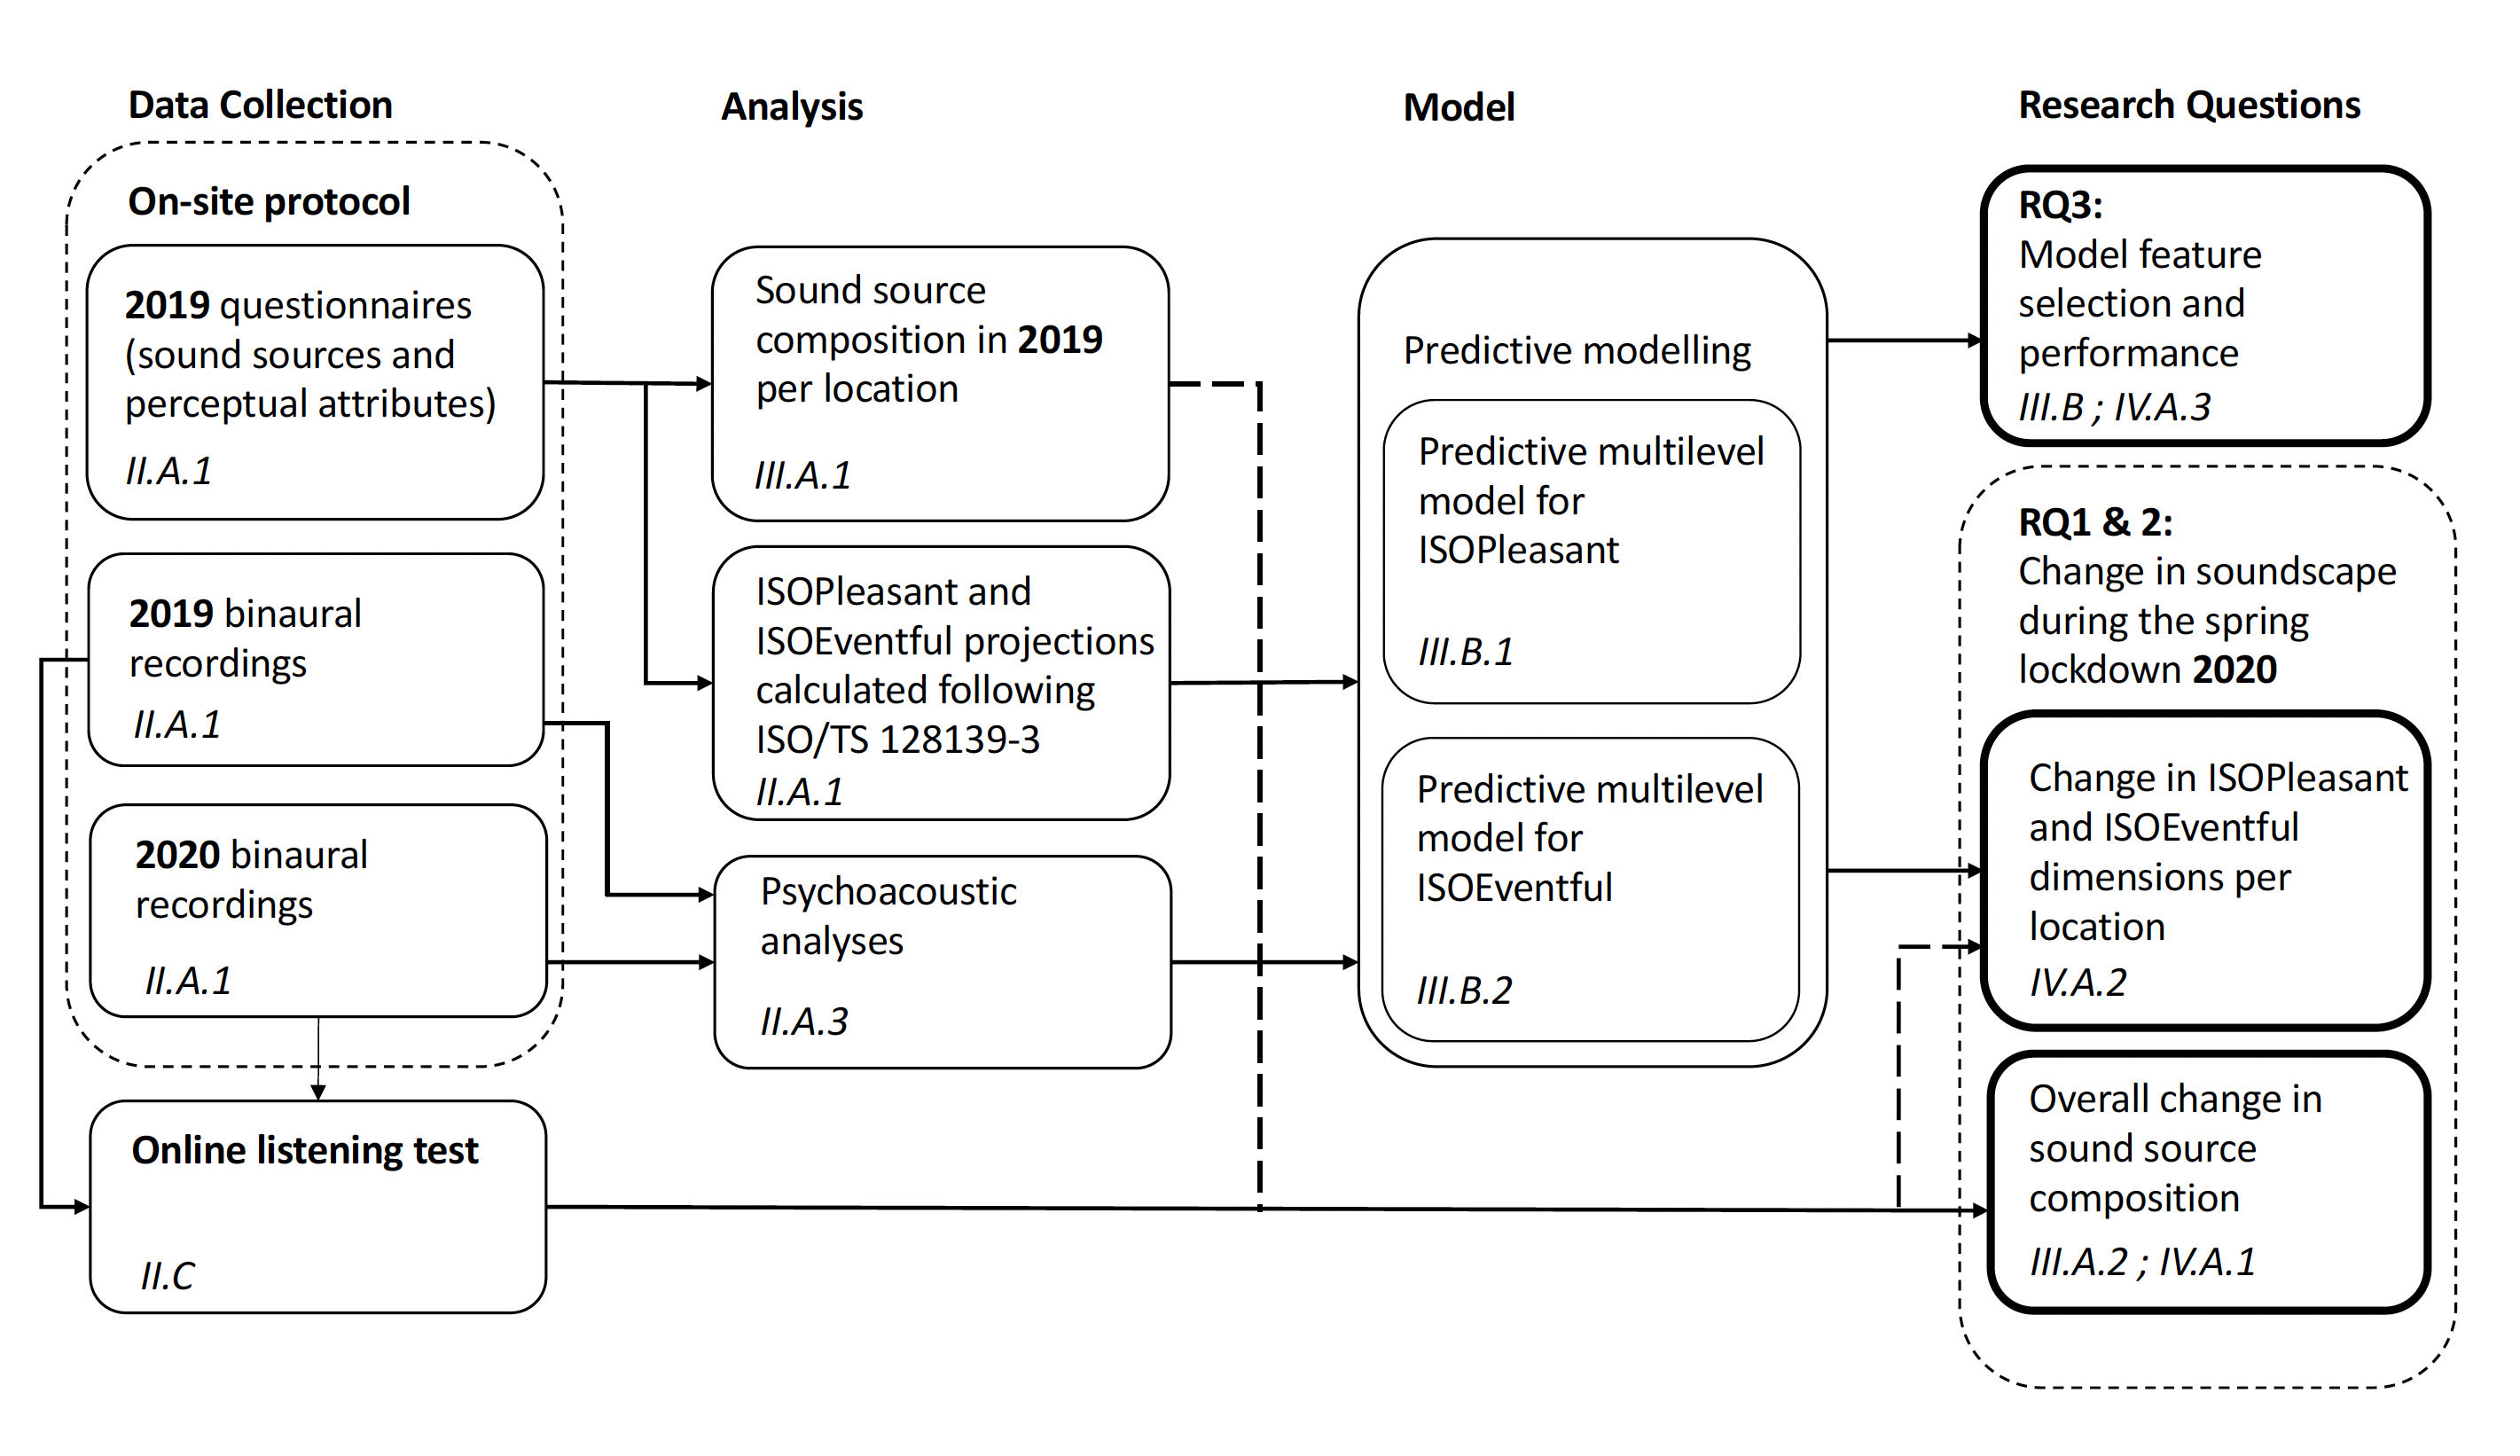
\includegraphics[width=1\textwidth,height=\textheight]{Figure1.png}

}

\caption{\label{fig-framework}The study flowchart indicating the data
collection, analysis, modeling, and discussion throughout the study. The
subsections in the text to which each box refers are indicated in
italics.}

\end{figure}%

\section{Results}\label{results}

The results of the onsite surveys, online experiment, and the model
development are reported here. They are reported following the structure
of the ISO/TS 12913 series, revealing the perceived sound source
dominance, key perceptual attributes (ISOPleasant and ISOEventful) and
the lockdown-related changes.

\subsection{Perceived sound source
dominance}\label{perceived-sound-source-dominance}

\subsubsection{2019 sound source composition per
location}\label{sound-source-composition-per-location}

Questionnaire data was collected in English, Italian, and Spanish in
both cities. The respective questionnaires can be found in the
supplementary files and \citet{Mitchell2020Soundscape}. Data presented
here was aggregated per LocationID.

According to the highest scored mean value of the dominant sound source
type, as shown in Figure~\ref{fig-barchart}, the locations can be
grouped into: natural sounds dominated (RegentsParkJapan,
RegentsParkFields, RussellSq), human sounds dominated (SanMarco,
TateModern, StPaulsRow, StPaulsCross, MonumentoGaribaldi), noise
(traffic and other noise) sounds dominated (CamdenTown, EustonTap,
TorringtonSq, PancrasLock). Traffic noise and Other noise have been
combined here, and for the rest of the discussion, as these responses
are highly correlated within this dataset and it is not helpful to
consider them separately for this analysis. This follows the alternative
sound source labels given in Figure C.3 of \citet{ISO12913Part2} which
combines Traffic and Other Noise. Finally, MarchmontGarden is unique in
that all sound source types are assessed as being nearly equally
present, with only 0.2 separating the least present (Other noise, 2.5)
and the most present (Traffic noise, 2.7).

\begin{figure}

\centering{

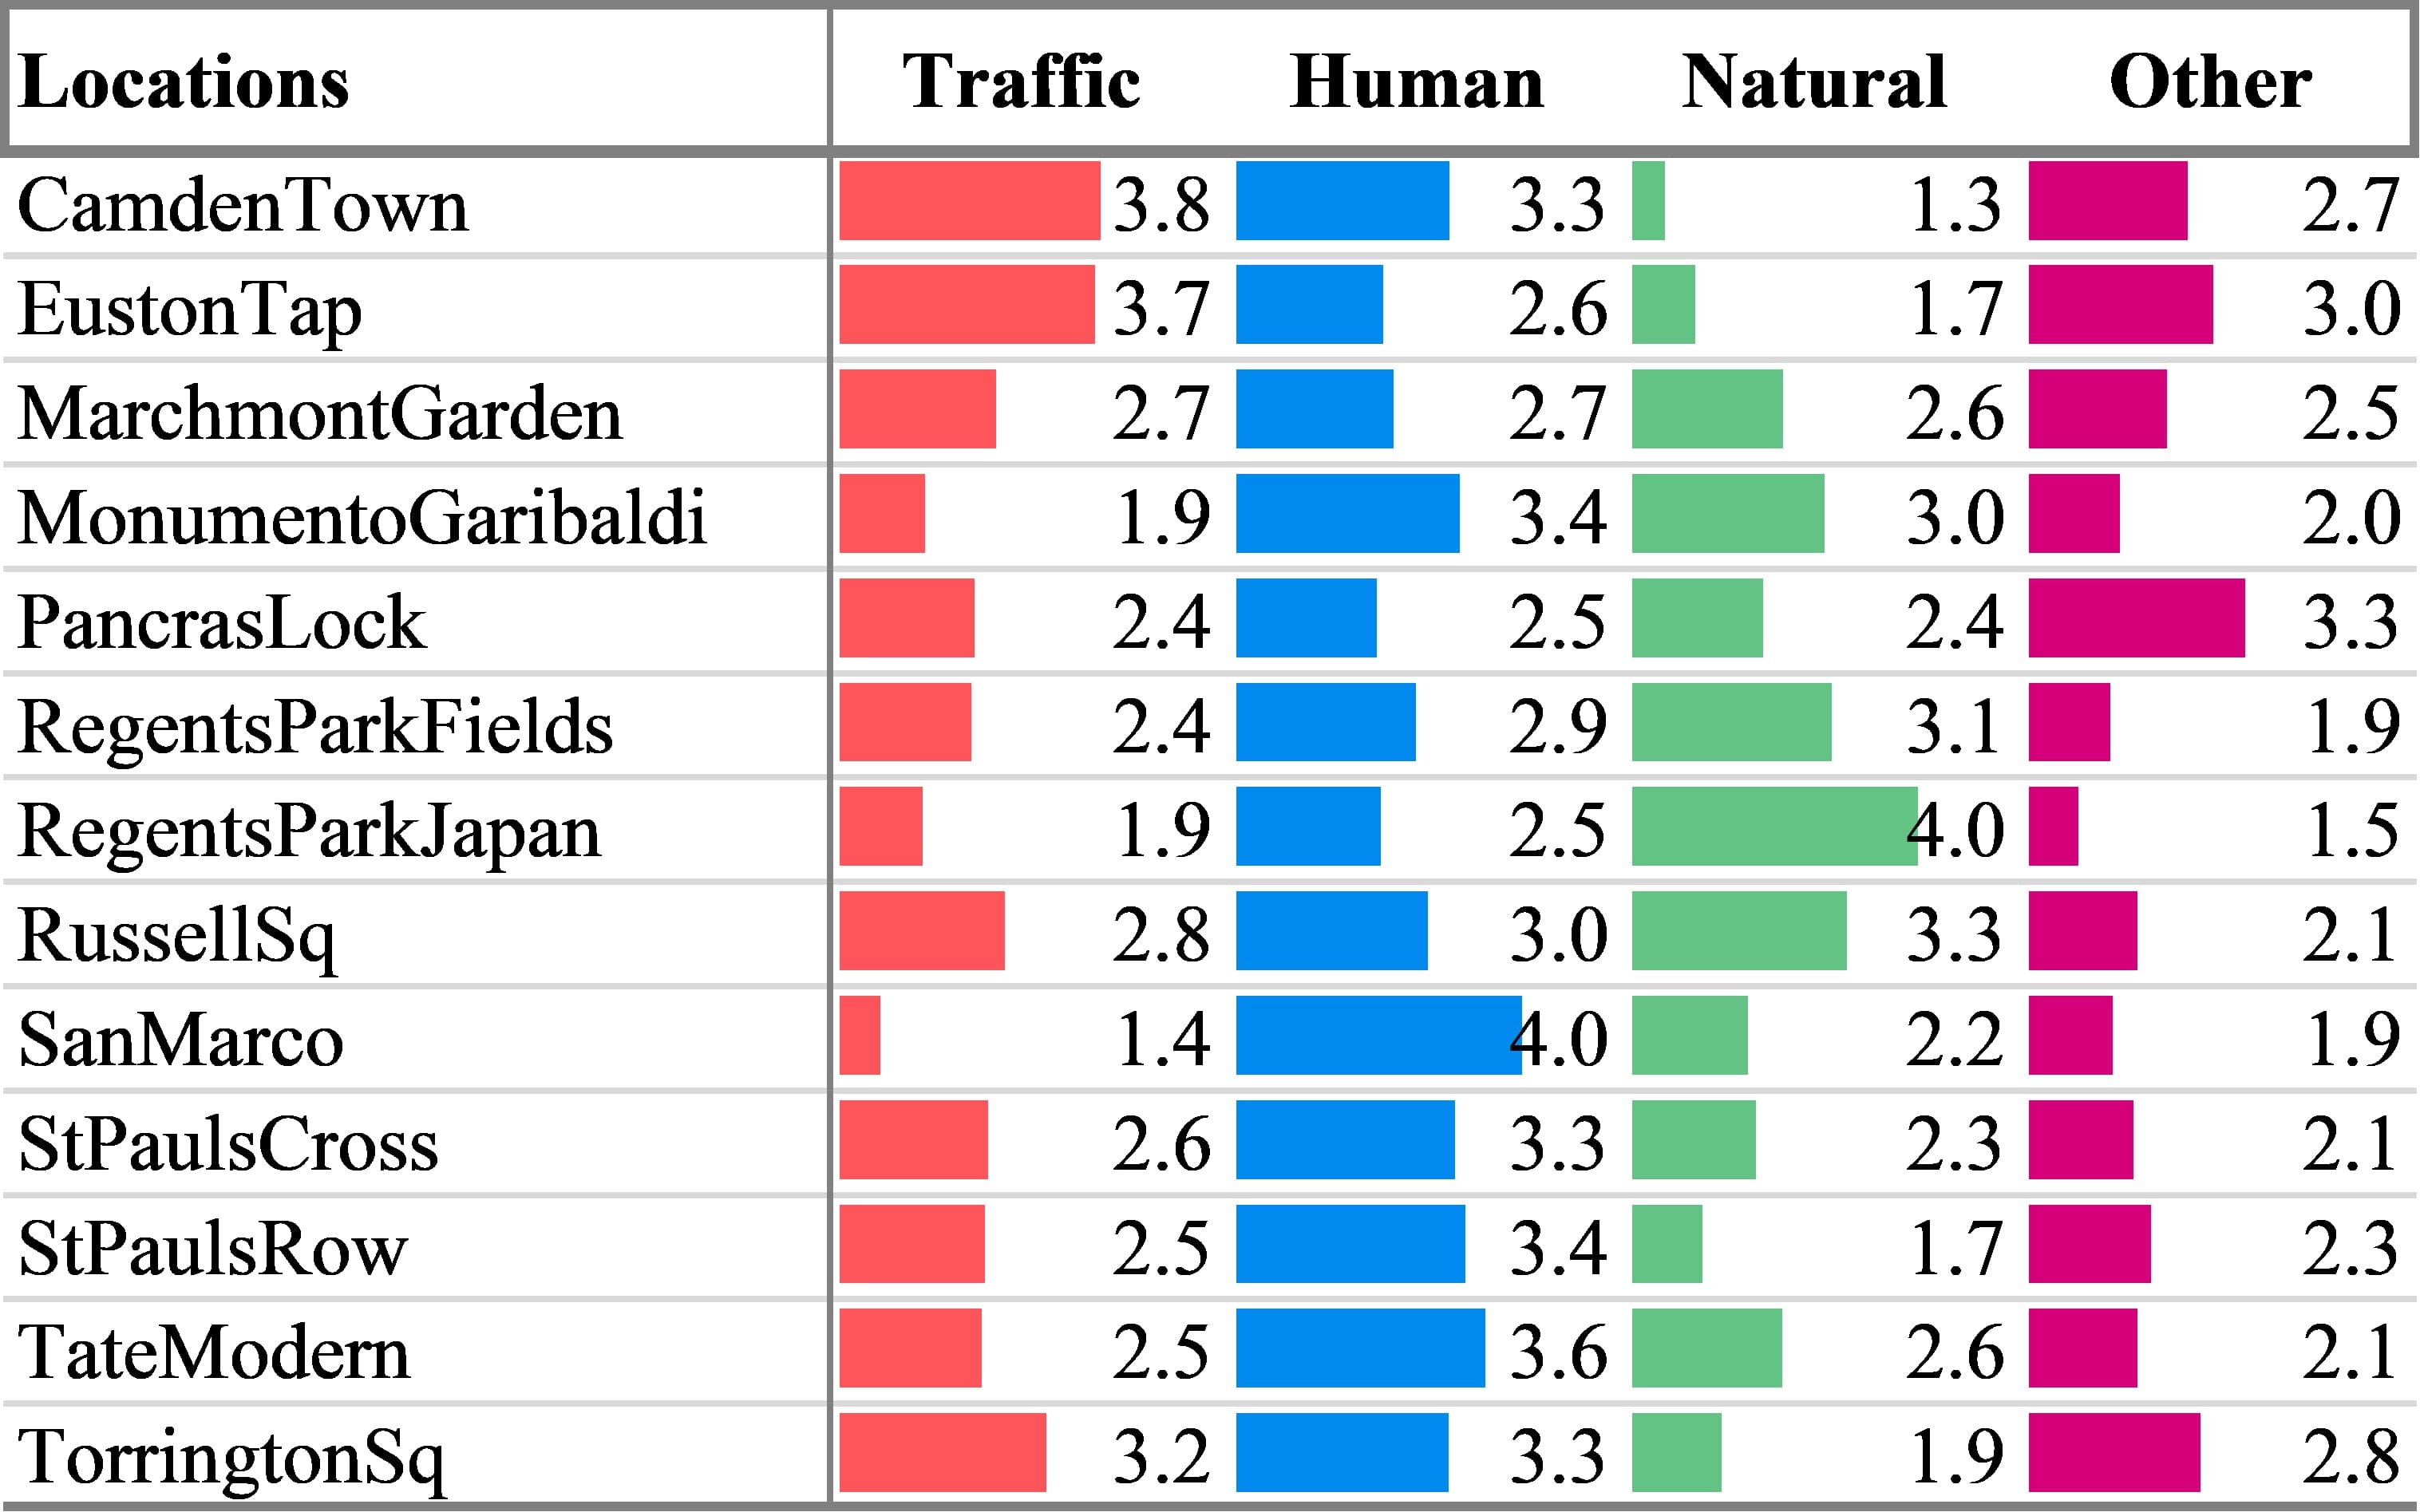
\includegraphics[width=0.6\textwidth,height=\textheight]{Figure2.jpg}

}

\caption{\label{fig-barchart}(Color online) Mean response per Location
ID for the perceived dominance of the sound source types, for the 2019
on-site campaign. The values represent the mean response of all
participants in each location to the question ``To what extent do you
presently hear the following four types of sounds?''. Response values
range from {[}1{]} Not at all to {[}5{]} Dominates completely.}

\end{figure}%

\subsubsection{Overall change in the perceived sound source dominance
during
lockdown}\label{overall-change-in-the-perceived-sound-source-dominance-during-lockdown}

1803 words describing the sound sources present in the 2019 recordings
and 1395 words related to the 2020 recordings were input by participants
in response to the open-ended question Q1 (see Appendix A). The
frequency of occurrence, generated using the WordClouds web app, is
shown in the Figure~\ref{fig-wordclo}, for the 2019 and the 2020 sets
respectively. The most frequent words from both 2019 and 2020 groups
are: noise, car/traffic, bird/birds, talk/voice and (foot)steps.

\begin{figure}

\begin{minipage}[t]{0.25\linewidth}
~\end{minipage}%
%
\begin{minipage}[t]{0.50\linewidth}

\raisebox{-\height}{

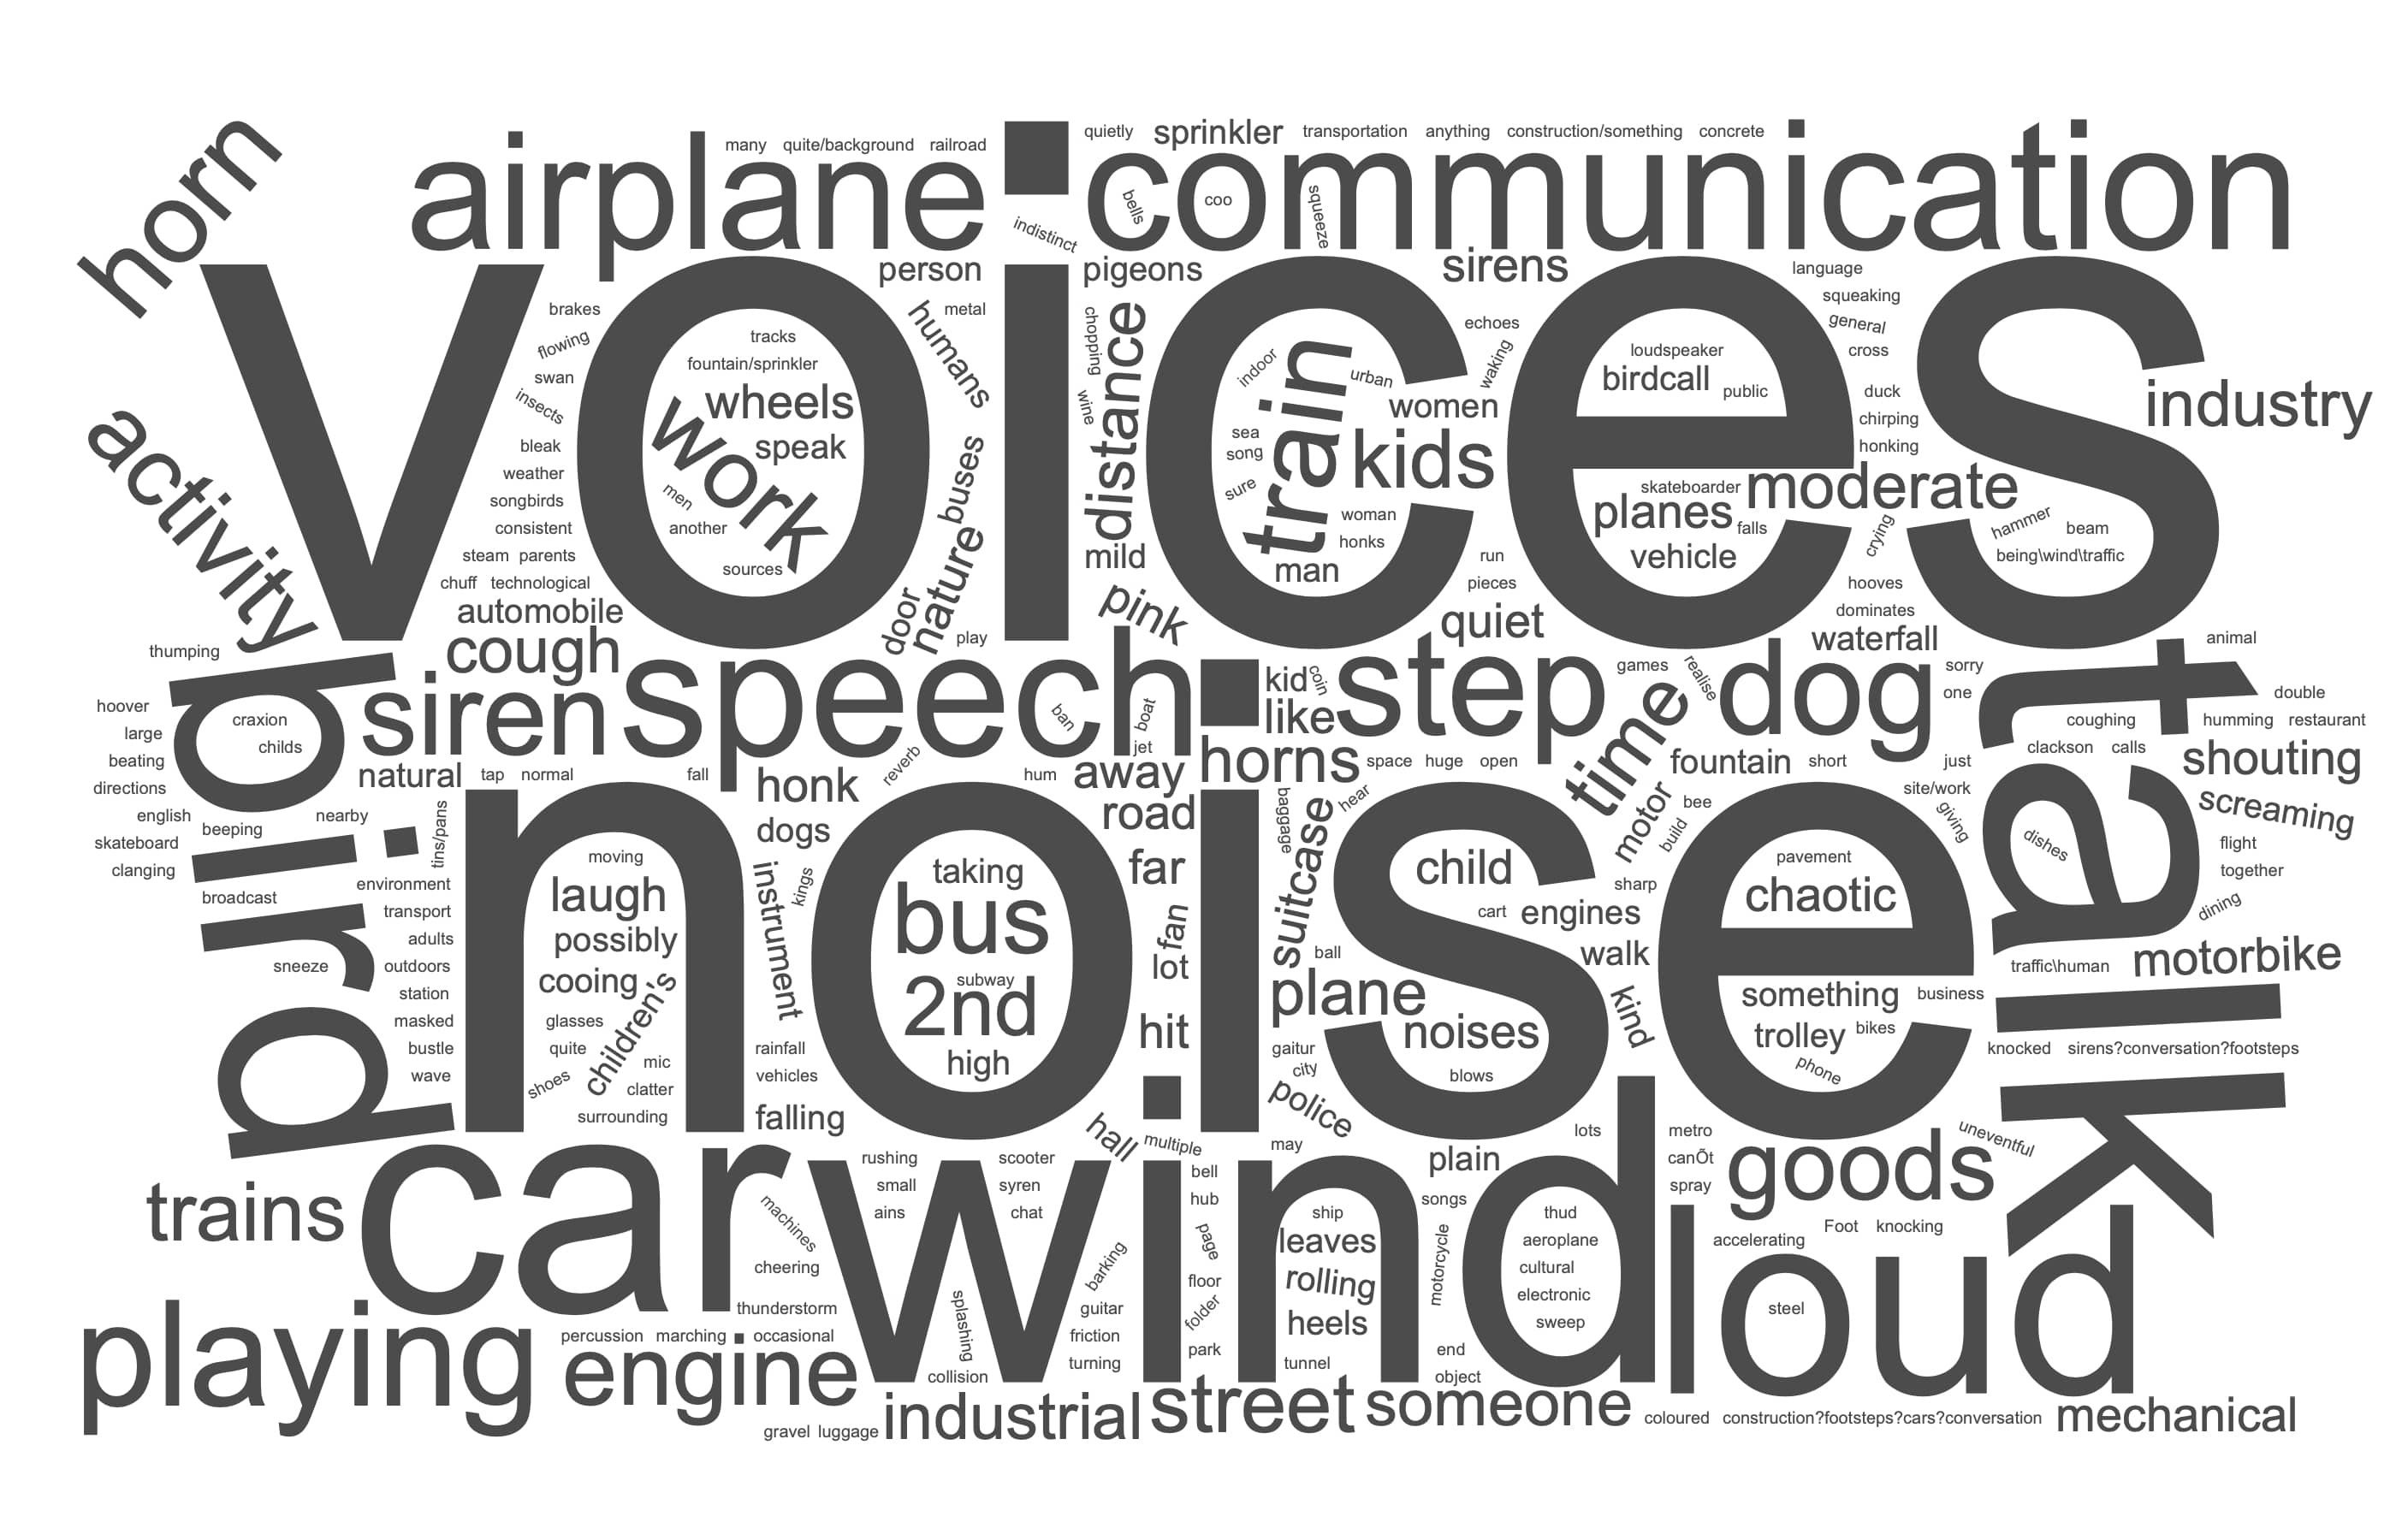
\includegraphics{Figure3a.jpg}

}

\end{minipage}%
%
\begin{minipage}[t]{0.25\linewidth}
~\end{minipage}%
\newline
\begin{minipage}[t]{0.25\linewidth}
~\end{minipage}%
%
\begin{minipage}[t]{0.50\linewidth}

\raisebox{-\height}{

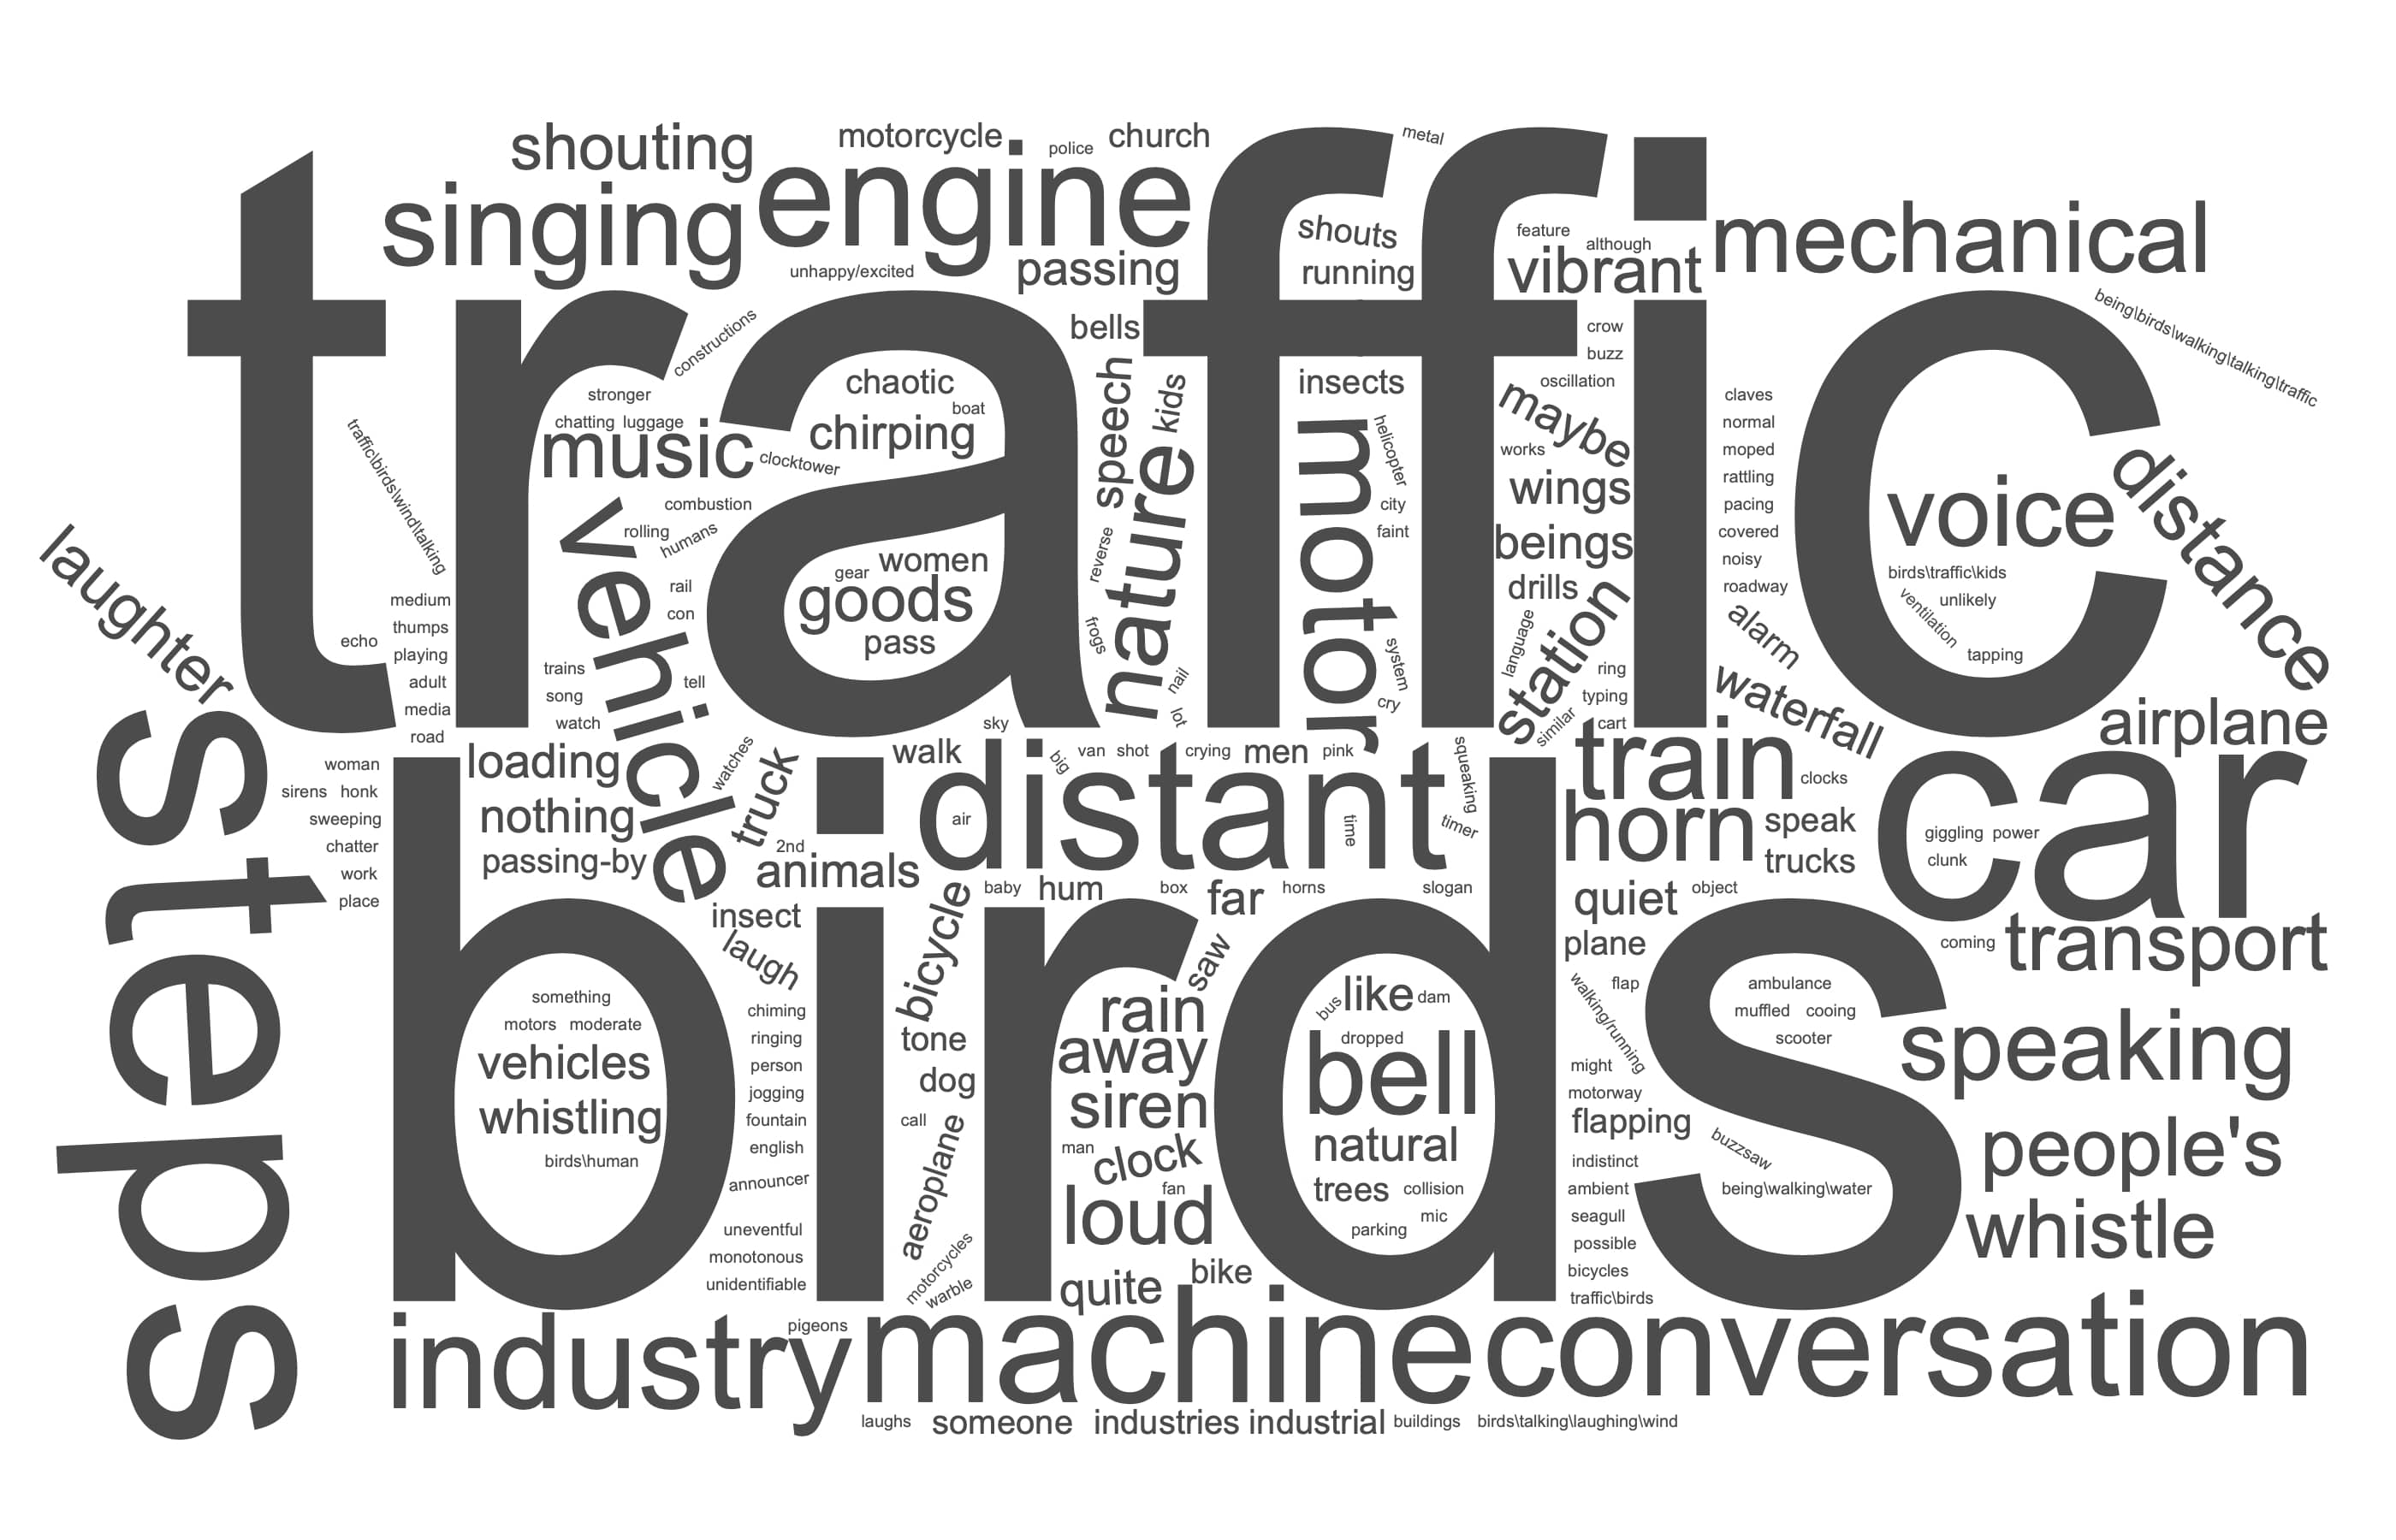
\includegraphics{Figure3b.jpg}

}

\end{minipage}%
%
\begin{minipage}[t]{0.25\linewidth}
~\end{minipage}%

\caption{\label{fig-wordclo}A graphic illustrating the frequency of
occurrence of the sound sources reported by the participants of the
online study across all locations, shown for recordings from the 2019
(above) and 2020 (below).}

\end{figure}%

The results from the listening tests deployed online were analyzed using
the SPSS Statistics v. 25. Levene's test for equality of variances
resulted in highly statistically significant values for all 4 sound
sources investigated (less than 0.001). Therefore, a Mann-Whitney U-test
test was used as a non-parametric equivalent to the T-test to
investigate the change in the perceived dominance of the four sound
source types \citep{McKnight2010Mann}. The results for human sounds
indicated that the perceived dominance was greater for the 2019 sample
(M=3.82), than for the 2020 sample (M=2.62), U=41,656, p \textless{}
0.001. The results for natural sounds indicated the perceived dominance
increased from 2019 (M=2.00) to 2020 (M=2.54), U=63,797, p \textless{}
0.001. However, the differences for the noise sources (traffic and
other) were not statistically significant. The result of these changes
is that while Human sounds were the clearly dominant source across the
whole dataset in 2019, in 2020 the sound sources are, on average, much
more evenly balanced. No single sound source category was identified as
frequent across the 2020 dataset.

\begin{longtable}[]{@{}
  >{\raggedright\arraybackslash}p{(\columnwidth - 10\tabcolsep) * \real{0.2346}}
  >{\centering\arraybackslash}p{(\columnwidth - 10\tabcolsep) * \real{0.1235}}
  >{\centering\arraybackslash}p{(\columnwidth - 10\tabcolsep) * \real{0.0617}}
  >{\centering\arraybackslash}p{(\columnwidth - 10\tabcolsep) * \real{0.0741}}
  >{\centering\arraybackslash}p{(\columnwidth - 10\tabcolsep) * \real{0.2469}}
  >{\centering\arraybackslash}p{(\columnwidth - 10\tabcolsep) * \real{0.2593}}@{}}
\caption{Mean values and standard deviation for the perceived dominance
of sound sources (rated from 1 - 5), assessed via an online
survey.}\label{tbl-source}\tabularnewline
\toprule\noalign{}
\begin{minipage}[b]{\linewidth}\raggedright
Sound source type
\end{minipage} & \begin{minipage}[b]{\linewidth}\centering
Campaign
\end{minipage} & \begin{minipage}[b]{\linewidth}\centering
N
\end{minipage} & \begin{minipage}[b]{\linewidth}\centering
Mean
\end{minipage} & \begin{minipage}[b]{\linewidth}\centering
Standard deviation
\end{minipage} & \begin{minipage}[b]{\linewidth}\centering
Standard error mean
\end{minipage} \\
\midrule\noalign{}
\endfirsthead
\toprule\noalign{}
\begin{minipage}[b]{\linewidth}\raggedright
Sound source type
\end{minipage} & \begin{minipage}[b]{\linewidth}\centering
Campaign
\end{minipage} & \begin{minipage}[b]{\linewidth}\centering
N
\end{minipage} & \begin{minipage}[b]{\linewidth}\centering
Mean
\end{minipage} & \begin{minipage}[b]{\linewidth}\centering
Standard deviation
\end{minipage} & \begin{minipage}[b]{\linewidth}\centering
Standard error mean
\end{minipage} \\
\midrule\noalign{}
\endhead
\bottomrule\noalign{}
\endlastfoot
Traffic & 2019 & 422 & 2.51 & 1.369 & 0.067 \\
& 2020 & 383 & 2.56 & 1.525 & 0.078 \\
Other & 2019 & 422 & 2.00 & 1.182 & 0.058 \\
& 2020 & 382 & 2.23 & 1.333 & 0.068 \\
Human & 2019 & 423 & 3.82 & 1.143 & 0.056 \\
& 2020 & 382 & 2.62 & 1.346 & 0.069 \\
Natural & 2019 & 424 & 2.00 & 1.307 & 0.063 \\
& 2020 & 380 & 2.54 & 1.441 & 0.074 \\
\end{longtable}

\subsection{Model selection, performance, and
application}\label{model-selection-performance-and-application}

\begin{longtable}[]{@{}
  >{\raggedright\arraybackslash}p{(\columnwidth - 12\tabcolsep) * \real{0.1538}}
  >{\raggedright\arraybackslash}p{(\columnwidth - 12\tabcolsep) * \real{0.2846}}
  >{\raggedright\arraybackslash}p{(\columnwidth - 12\tabcolsep) * \real{0.2077}}
  >{\raggedright\arraybackslash}p{(\columnwidth - 12\tabcolsep) * \real{0.1000}}
  >{\raggedright\arraybackslash}p{(\columnwidth - 12\tabcolsep) * \real{0.1000}}
  >{\raggedright\arraybackslash}p{(\columnwidth - 12\tabcolsep) * \real{0.0923}}
  >{\raggedright\arraybackslash}p{(\columnwidth - 12\tabcolsep) * \real{0.0615}}@{}}
\caption{Scaled linear regression models of ISOPleasant and ISOEventful
for 13 locations in London and Venice. ISOPleasant model structure:
Random slope, random intercept multi-level model. ISOEventful model
structure: Multi-variate linear
regression.}\label{tbl-model}\tabularnewline
\toprule\noalign{}
\begin{minipage}[b]{\linewidth}\raggedright
\end{minipage} & \begin{minipage}[b]{\linewidth}\raggedright
ISOPleasant
\end{minipage} & \begin{minipage}[b]{\linewidth}\raggedright
\end{minipage} & \begin{minipage}[b]{\linewidth}\raggedright
\end{minipage} & \begin{minipage}[b]{\linewidth}\raggedright
ISOEventful
\end{minipage} & \begin{minipage}[b]{\linewidth}\raggedright
\end{minipage} & \begin{minipage}[b]{\linewidth}\raggedright
\end{minipage} \\
\midrule\noalign{}
\endfirsthead
\toprule\noalign{}
\begin{minipage}[b]{\linewidth}\raggedright
\end{minipage} & \begin{minipage}[b]{\linewidth}\raggedright
ISOPleasant
\end{minipage} & \begin{minipage}[b]{\linewidth}\raggedright
\end{minipage} & \begin{minipage}[b]{\linewidth}\raggedright
\end{minipage} & \begin{minipage}[b]{\linewidth}\raggedright
ISOEventful
\end{minipage} & \begin{minipage}[b]{\linewidth}\raggedright
\end{minipage} & \begin{minipage}[b]{\linewidth}\raggedright
\end{minipage} \\
\midrule\noalign{}
\endhead
\bottomrule\noalign{}
\endlastfoot
Predictors & Estimates & Confidence Interval (CI) & p & Estimates & CI &
p \\
(Intercept) & 0.24 & 0.15--0.33 & \textless0.001 & 0.14 & 0.12--0.16 &
\textless0.001 \\
N5 & −0.06 & −0.10--0.02 & \textless0.001 & & & \\
S & & & & −0.08 & −0.11--0.06 & \textless0.001 \\
FS & & & & −0.02 & −0.05--0.00 & 0.033 \\
T & & & & 0.04 & 0.01--0.07 & 0.002 \\
\(L_{Aeq}\) & & & & 0.14 & 0.11--0.17 & \textless0.001 \\
\(L_{Ceq}-L_{Aeq}\) & & & & −0.03 & −0.05--0.00 & 0.052 \\
\textbf{Random effects} & & & & & & \\
\(\sigma^2\) & 0.11 & & & & & \\
\(\tau_{00}\) & \(0.03_{LocationID}\) & & & & & \\
\(\tau_{11}\) & \(0.02_{LocationID.L_{Aeq}}\) & & & & & \\
& \(0.00_{LocationID.L_{A10}-L_{A90}}\) & & & & & \\
& \(0.00_{LocationID.L_{Ceq}-L_{Aeq}}\) & & & & & \\
ICC & 0.90 & & & & & \\
N & \(13_{LocationID}\) & & & & & \\
Observations & 914 & & & 914 & & \\
MAE train, test & 0.258 & 0.259 & & 0.233 & 0.231 & \\
\end{longtable}

\subsubsection{ISOPleasant model
selected}\label{isopleasant-model-selected}

Following the feature selection, the ISOPleasant model (given in
Table~\ref{tbl-model}) has \(N_5\) as the fixed effect with a scaled
coefficient of -0.06, and \(L_{Aeq}\), \(L_{A10}-L_{A90}\), and
\(L_{Ceq}-L_{Aeq}\) as coefficients which vary depending on the
LocationID. The training and testing MAE are very similar, indicating
that the model is neither over- nor under-fitting to the training data
(\(MAE_{train} = 0.258\); \(MAE_{test} = 0.259\)). The model performs
very well at predicting the average soundscape assessment of the
locations (\(R^2_{train} = 0.998\); \(R^2_{test} = 0.85\)).

The high intraclass correlation (\(ICC = 0.90\)) demonstrates that the
location-level effects are highly important in predicting the
pleasantness dimension. Within this random-intercept random-slope model
structure, these effects include both the specific context of the
location (i.e.~the LocationID factor), but also the \(L_{Aeq}\),
\(L_{A10}-L_{A90}\), and \(L_{Ceq}-L_{Aeq}\) features whose effects vary
across locations. These slopes are given in Figure~\ref{fig-random}.
This point highlights the need to consider how the context of a location
will influence the relationship between the acoustic features and the
perceived pleasantness.

\begin{figure}

\centering{

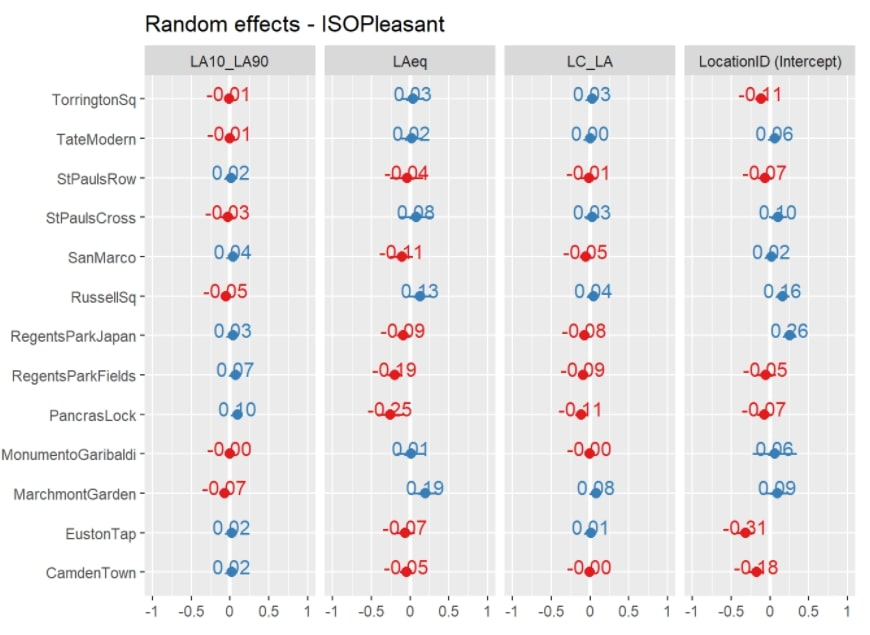
\includegraphics[width=0.75\textwidth,height=\textheight]{Figure4.jpg}

}

\caption{\label{fig-random}(Color online) Location-level scaled
coefficients for the ISOPleasant model.}

\end{figure}%

\subsubsection{ISOEventful model
selected}\label{isoeventful-model-selected}

Through the group-level feature selection, all of the group-level
coefficients were removed, including the LocationID factor itself.
Therefore the final ISOEventful model is a `flat' multi-variate linear
regression model, rather than a multi-level model. The ISOEventful model
is a linear combination of S, FS, T, \(L_{Aeq}\), and
\(L_{Ceq}-L_{Aeq}\). The training and testing MAE are very similar,
indicating that the model is not over-fit to the training data
(\(MAE_{train} = 0.233\); \(MAE_{test} = 0.231\)). The model performs
slightly worse than the ISOPleasant at predicting the mean location
responses, but still performs well (\(R^2_{train} = 0.873\);
\(R^2_{test} = 0.715\)).

\subsubsection{Application to lockdown data}\label{sec-application}

\begin{figure}

\centering{

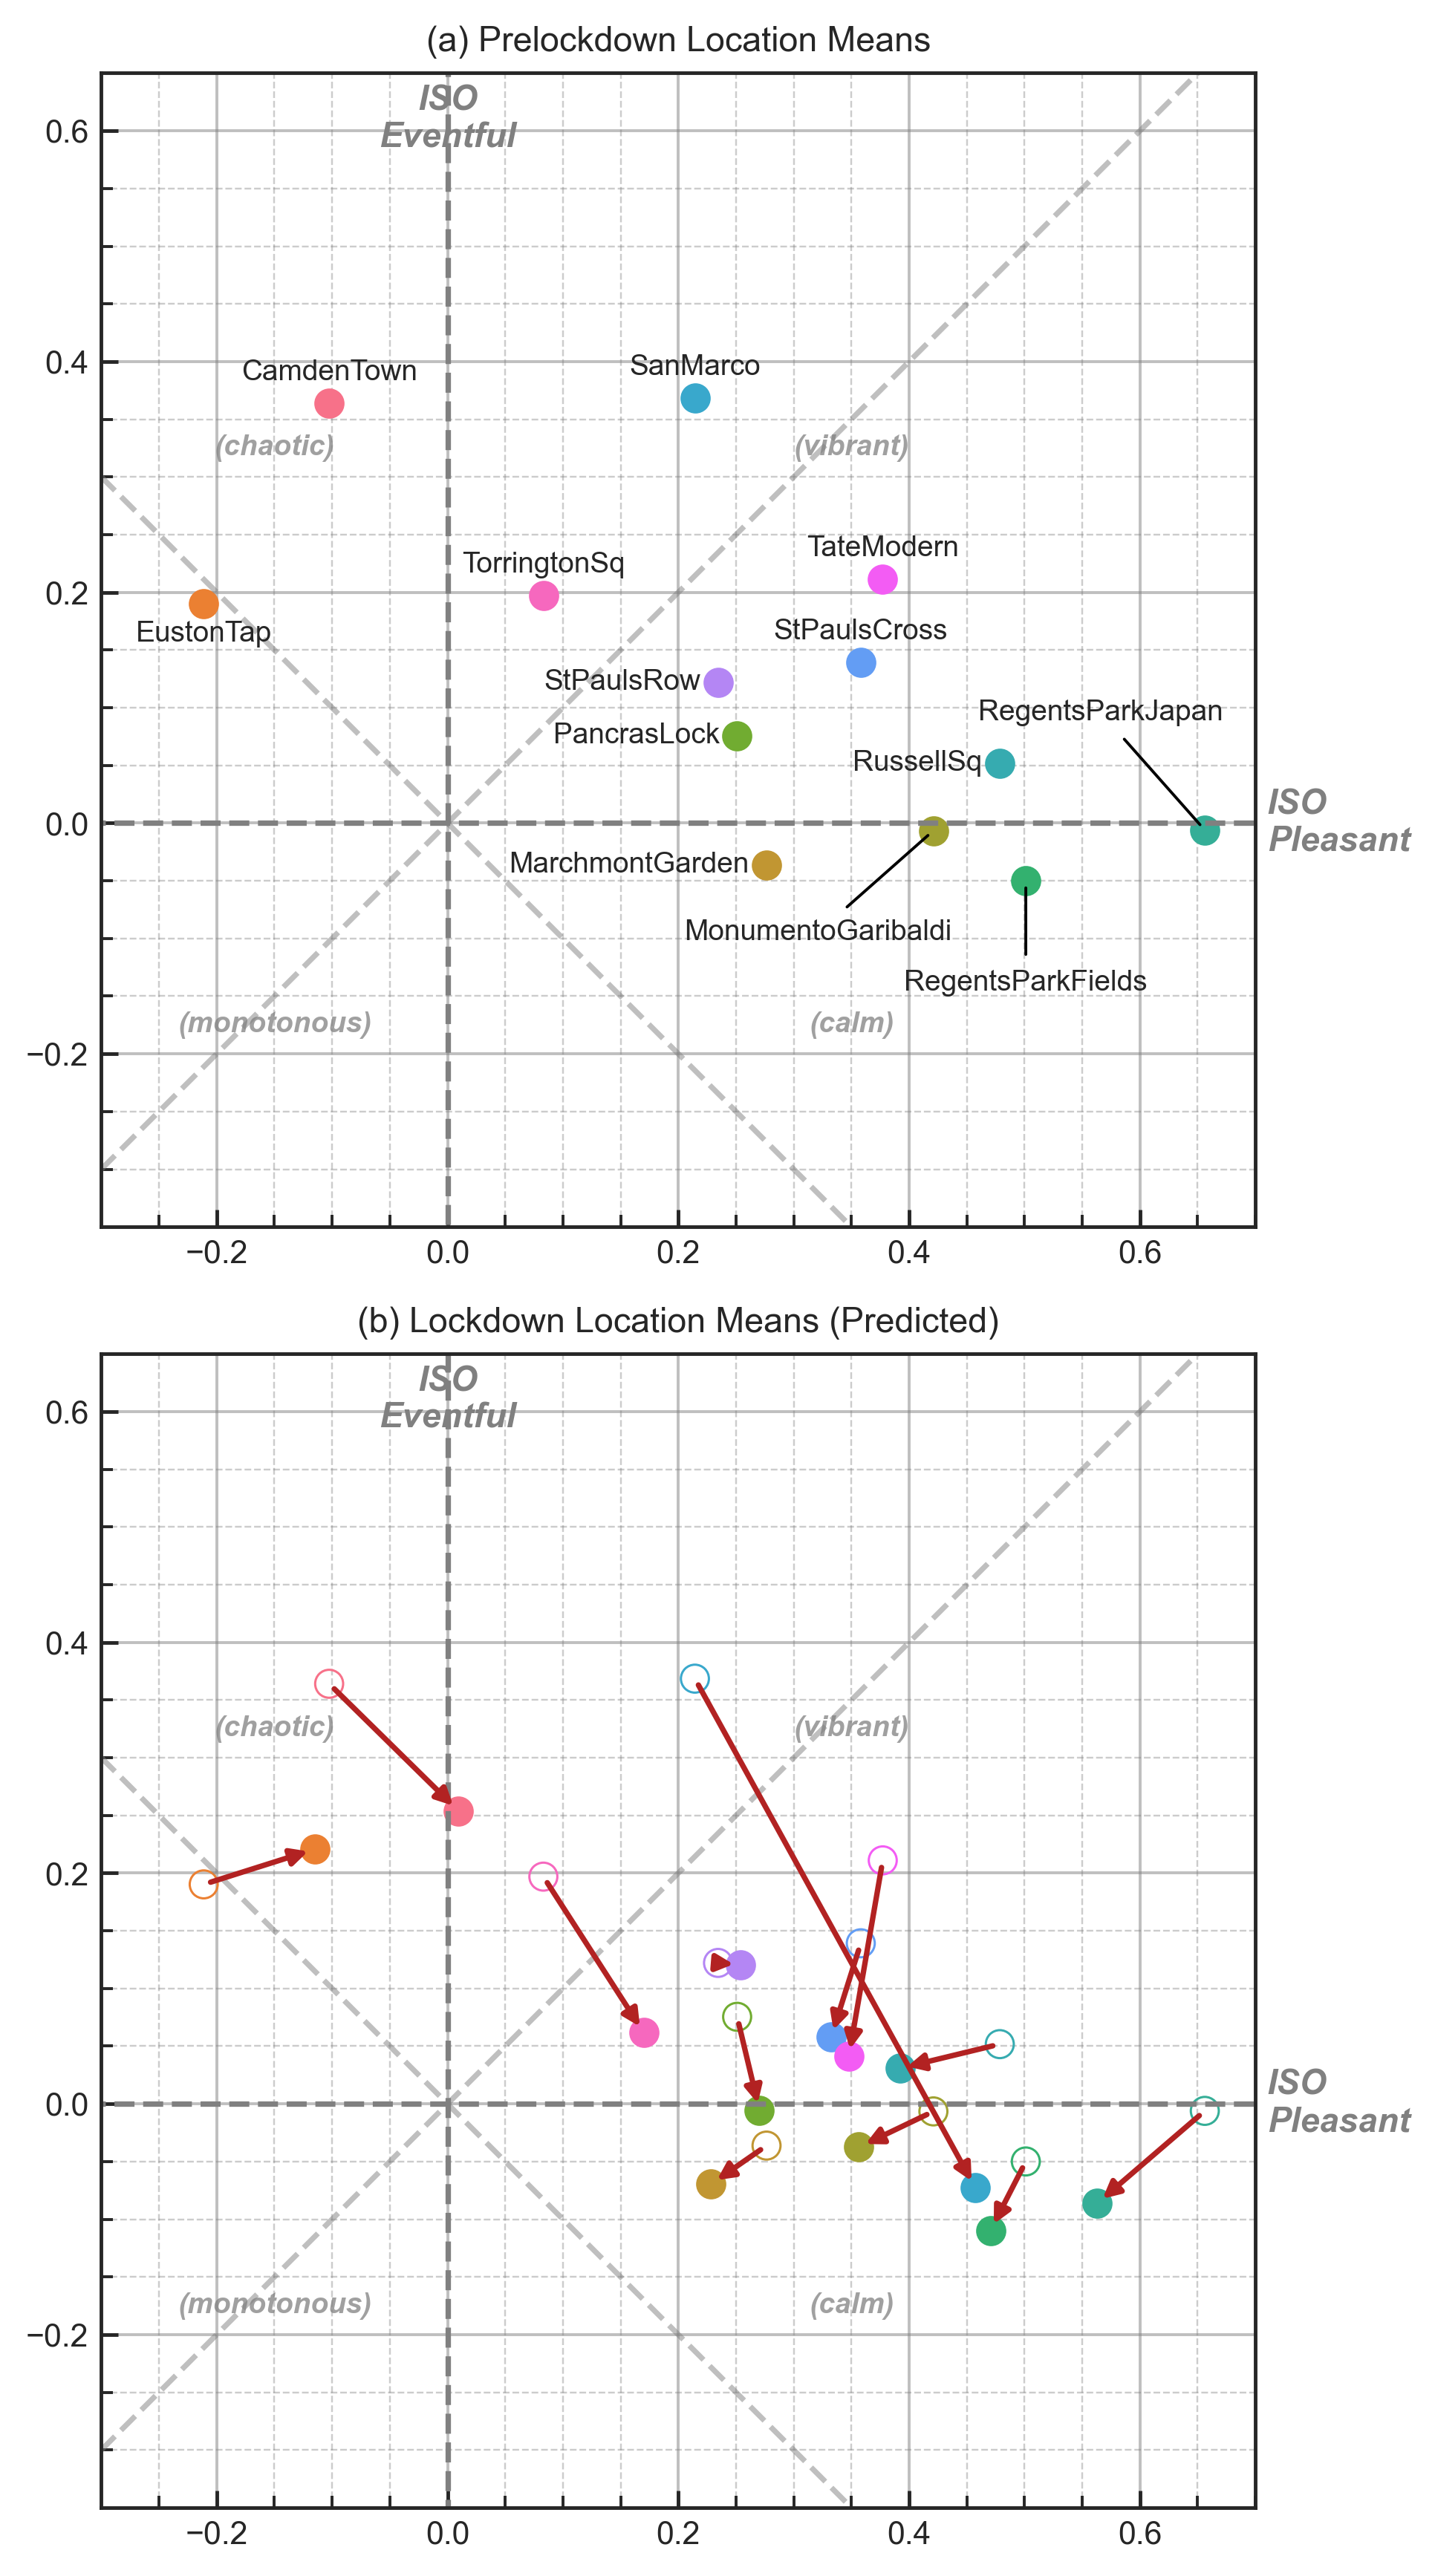
\includegraphics[width=0.75\textwidth,height=\textheight]{Figure5.jpg}

}

\caption{\label{fig-locations}(Color online) Soundscape circumplex
coordinates for (a) the mean ISOPleasant and ISOEventful responses for
each location; and (b) the mean predicted responses based on recordings
made during the lockdown and the change in the location's placement in
the circumplex. In (b) the marker outline is shown for the 2019
location, red arrows indicate the change in the location's coordinates.}

\end{figure}%

Once the two models were built and assessed, they were then applied to
the lockdown recording data in order to predict the new soundscape ISO
coordinates. Figure~\ref{fig-locations} (a) shows the pre-lockdown ISO
coordinates for each location and Figure~\ref{fig-locations} (b) shows
how the soundscapes are predicted to have been assessed during the
lockdown period. As in the model assessment process, the predicted
responses are calculated for each recording individually, then the mean
for each location is calculated and plotted on the circumplex.

In 2019 the majority of locations in the dataset fall within the
`vibrant' quadrant of the circumplex, particularly those which are
primarily dominated by human activity (e.g.~San Marco, Tate Modern).
Camden Town and Euston Tap, which are both in general visually and
acoustically dominated by traffic, are the only two to be rated as
`chaotic', while no locations are overall considered to be `monotonous'.
During the 2020 lockdown, there is general positive move along the
`pleasant' dimension and general negative move along the `eventful'
dimension, but several different patterns of movement can be noted.
These are investigated further in the Discussion section below.

\section{Discussion}\label{discussion}

\subsection{Interpretation of the
results}\label{interpretation-of-the-results}

To interpret the results addressing the RQ1 and RQ2, it is necessary to
separately look into the overall change in sound source composition, and
the change in the affective quality of soundscapes per location.

\subsubsection{Change in the sound source
composition}\label{change-in-the-sound-source-composition}

The open-ended question about sound sources in the online survey did not
reveal a change in sound source types but rather confirmed that all
types were still present in both conditions. The sound source
composition question taken from the Method A of the
\citet{ISO12913Part2} revealed a statistically significant reduction in
human sound sources and a significant increase in the perceived
dominance of natural sound sources.

The most frequent sound sources detected from the open-ended question
correspond to the main four sound source types investigated, which
indicated that all types remained present in the lockdown condition (at
all the locations). While traffic intensity might have gone down, where
the results of the Mann-Whitney U-test were inconclusive, but supported
by the psychoacoustic measurements \citep{Aletta2020Assessing},
traffic-related sound sources were still clearly present.

The sound source composition of an outdoor acoustic environment is
extremely complex. Removing one component, such as human sounds, has
implications on the whole \citep{Gordo2021Rapid}. Testing the effects of
this in situ is not straightforward and interpreting this study in line
with `what is the impact of human sounds' must be taken within the
broader context of the range of conditions which changed within the
acoustic environment. However, looking at the overarching picture, the
lockdown condition was a useful and unique case study to understand the
impact which human activities -- and the human sound source type in
particular -- can have on soundscape perception of urban open spaces.

\subsubsection{Predicted relative changes in soundscapes due to COVID-19
restrictions}\label{predicted-relative-changes-in-soundscapes-due-to-covid-19-restrictions}

\begin{figure}

\centering{

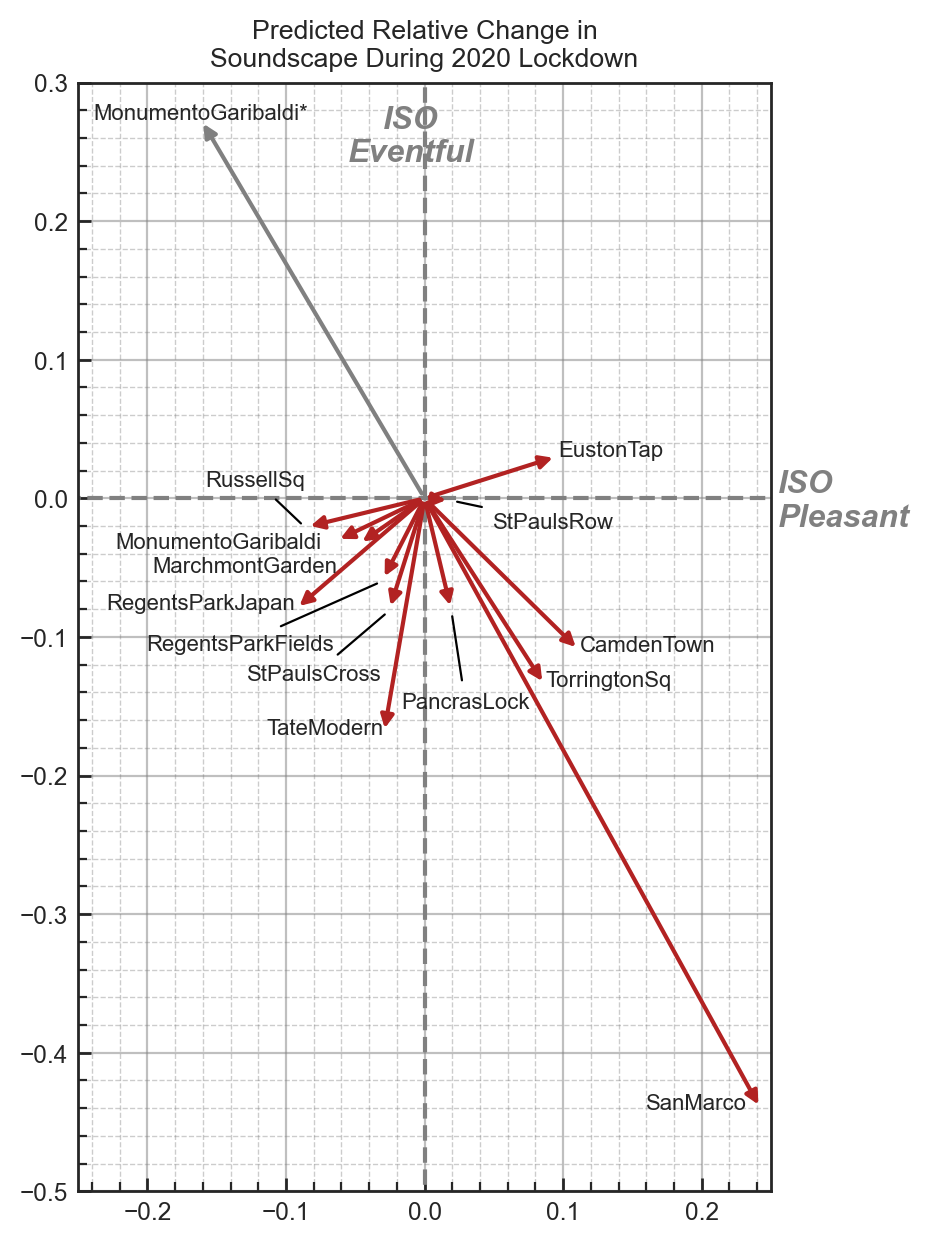
\includegraphics{Figure6.jpg}

}

\caption{\label{fig-vectors}(Color online) The relative change in
soundscape perception in the circumplex due to the COVID-19 lockdowns as
predicted by the models, represented as vectors centered on the origin.
\emph{The lawn-works dominated session is shown separately as
MonumentoGaribaldi} with a gray arrow to indicate that this is distinct
from the effects of the lockdown changes.}

\end{figure}%

In order to interpret how the change of the acoustic environment at the
locations examined would have been perceived, and to answer RQ2,
relative change vectors within the circumplex space are shown in Figure
\ref{fig:vectors}. This clearly shows a few different patterns of
soundscape change due to the effects of the 2020 lockdown. These can be
further looked into depending on the magnitude and direction of change,
shifts between quadrants shown in Figure~\ref{fig-locations}, and the
sound source composition. The discussion below is organized according to
groups of locations which show similar behaviors in the predicted
magnitude and direction of change, or discusses a single location which
is particularly notable.

\paragraph{Piazza San Marco}\label{piazza-san-marco}

The largest change is seen in Piazza San Marco, with a predicted
increase in pleasantness of 0.24 and a decrease in eventfulness of 0.44,
enough to move the soundscape out of the `vibrant' quadrant and into
`calm'. This extreme change (relative to the rest of the locations) is
exactly what would be expected given the unique context of the
measurements taken in 2019 -- the measurement campaign corresponded with
Carnevale, a yearly festival which centers around the square. By
contrast, due to the particularly strict measures imposed in Italy,
during the lockdown measurement period, the square was almost entirely
devoid of people. What is promising is that, without any of this
contextual information about the presence or absence of people, our
model is able to capture and reflect what may be considered a reasonable
and expected direction and scale of change within the soundscape
circumplex.

\paragraph{Locations showing an increase in
pleasantness}\label{locations-showing-an-increase-in-pleasantness}

The next locations of interest are those which, in the 2019 survey data,
were rated as being dominated by traffic noise: Euston Tap, Camden Town,
Torrington Square, and Pancras Lock. These are the only locations
(besides San Marco) which show a predicted increase in pleasantness. Of
these traffic-dominated spaces, the two which were most heavily
dominated by traffic noise (Camden Town and Euston Tap) showed the most
increase in pleasantness, with Torrington Square having slightly less of
an increase. Pancras Lock, which was also rated as having high levels of
both Human and Natural sounds shows only a modest improvement in
pleasantness.

\paragraph{Locations showing a decrease in
pleasantness}\label{locations-showing-a-decrease-in-pleasantness}

Among the locations which are predicted to experience a negative effect
on pleasantness we see a mix of spaces which were assessed as being
dominated by Human (St Pauls Cross and Tate Modern) and Natural (Regents
Park Japan, Regents Park Fields, Russell Square) sounds before the
lockdown. It is hard to discern a pattern of difference between these
two groups, although it appears that the Human-dominated spaces saw a
greater reduction in eventfulness, compared to the Natural-dominated
spaces.

In general, we note that most of the spaces experience some degree of
reduction in eventfulness. This pattern is particularly consistent with
what would be expected from a reduction in human presence in these
spaces \citep{Aletta2018Towards}, as reflected by the observation that,
in general, those spaces which had the most human sounds prior to the
lockdown showed the greatest reduction in eventfulness during the
lockdown. In particular, Tate Modern, Camden Town, and Torrington Square
show the greatest reduction in eventfulness. This appears to be due to
these locations showing the greatest reduction in overall \(L_{Aeq}\)
compared to other locations (8.1 dB, 5.2 dB, and 9.2 dB, respectively),
with \(L_{Aeq}\) being the most influential feature in the eventfulness
model, as shown in Table~\ref{tbl-model}. However, Russell Square also
experienced a large decrease in \(L_{Aeq}\) on average (10.5 dB) but
does not show the same reduction in eventfulness. This appears due to
the correspondingly large decrease in \(S\) (1.17 acum) which is not
seen at the 3 previously mentioned locations. Russell Square normally
features a medium-sized jet fountain which was turned off during the
lockdowns in 2020 and therefore it experienced a drop in the overall
sound level, but an increase in the proportion of low frequency noise to
high frequency noise reflected by a decrease in sharpness which, within
the eventfulness model, effectively cancels out the impact of the
reduction in \(L_{Aeq}\). While the overall sound level has an important
impact, in order to determine the true impact a reduction in sound level
may have, it must be taken in context with how the other aspects of the
sound will also change.

\paragraph{Euston Tap}\label{euston-tap}

An unexpected result is that Euston Tap is predicted to experience an
increase in eventfulness and it is unclear whether this accurately
reflects the real experience people would have had in the space.
Normally, Euston Tap is a mostly-outdoor drinking venue located at the
entrance to London Euston Station and situated directly along a very
busy central London road. During the 2020 survey, the researchers noted
that the music and chatter of people from the pub was noticeably
missing, but that the perceived reduction in road traffic was minimal.
Based on the theory of vibrancy which would suggest it is driven by
human presence and sounds \citep{Aletta2018Towards}, we would not
therefore expect a shift in the vibrant direction as indicated here.
This discrepancy may reveal a weakness in the context-independent
ISOEventful model, or it may in fact be indicating that, at certain
thresholds of traffic noise, a reduction in level -- and therefore a
reduction in energetic masking -- will allow other aspects of the sound
to influence the perception.

\paragraph{Monumento Garibaldi}\label{monumento-garibaldi}

Finally, special attention should be paid to the results shown for
Monumento Garibaldi, which in 2019 was perceived as a pleasant and
slightly calm green space featuring a gravel walkway. During the first
measurement session during the lockdown in 2020, the researcher noted
that the soundscape was dominated by landscaping works, in particular
noise from strimmers (or weed whackers). In order to gain a sample which
was more representative of the impact of the lockdowns, the researcher
returned another day to repeat the measurements without interference
from the works.

To examine the impact of these two scenarios separately, the prediction
model was fitted to the data from the two sessions independently and the
session which was impacted by the landscaping works is shown in
Figure~\ref{fig-vectors} in gray and labeled MonumentoGaribaldi*, while
the unaffected session is shown in red. In the latter case, the
predicted change in soundscape as a result of the lockdown fits neatly
into what would be expected and closely matches the predicted behavior
of similar locations in London (i.e.~Marchmont Garden and Russell
Square). On the other hand, the session which was dominated by noise
from the strimmers is predicted to have become much more chaotic, with a
decrease in pleasantness of 0.16 and an increase in eventfulness of
0.27. This indicates that, although the model has no contextual
information about the type of sound and in fact the training data never
included sounds from similar equipment, just based on the psychoacoustic
features of the sound it is able to reasonably predict the expected
change in soundscape.

\paragraph{General notes}\label{general-notes}

As a whole, the primary impact of the 2020 lockdowns on the soundscapes
in London and Venice was an overall decrease in eventfulness. With the
exception of Euston Tap, all of the sessions show some degree of
reduction in eventfulness, reflecting the general decrease in sound
levels and human sound sources across the locations. The impact of the
lockdowns on pleasantness is more mixed and seems to be driven by the
previous dominance of traffic noise in the space. However, it could also
be noted that, while all locations experienced a reduction in sound
level, those which are predicted to become more pleasant had an average
\(L_{Aeq}\) above 60 dB in 2019. By contrast, the locations which were
predicted to experience a decrease in pleasantness generally had sound
levels below 60 dBA in 2019. This may indicate that reductions in sound
level can improve pleasantness when the sound level exceeds some
threshold of around 60 - 65 dBA but are ineffective when sound levels
are below this threshold. Similarly, \citet{Yang2005Acoustic} showed
that, when the sound level is `lower than a certain value, say 70 dB'
there is no longer a significant improvement in the evaluation of
acoustic comfort as the sound level reduces. It is unclear at this point
where this threshold would lie for pleasantness/annoyance, how strict it
may be, or how it is impacted by the sound source composition of the
acoustic environment, therefore further research is needed in this area.

\subsubsection{Model selection results}\label{model-selection-results}

The most immediately interesting result of the model-building and
feature selection process, answering to RQ3, is the apparent irrelevance
of location context to the ISOEventful dimension. The multilevel model
structure was chosen since the starting assumption was that soundscape
perception is heavily influenced by contextual factors, such as
expectations of the space and visual context \citep{Ricciardi2015Sound}.
For this modeling, these factors can be considered as location-level
latent variables at least partially accounted for by the inclusion of
the LocationID as the second-level factor. While this assumption
certainly held true for ISOPleasant, our results indicate that these
types of contextual factors are not significant for ISOEventful, and do
not affect the relationship between the acoustic features of the sound
and the perception.

In particular this result may herald a shift in modeling approach for
soundscapes -- where previous methods, in both the soundscape and noise
paradigms, have mostly focused on deriving acoustic models of annoyance
(in other words have focused on the ISOPleasant dimension) perhaps they
should instead consider the acoustic models as primarily describing the
eventfulness dimension when considered in situ. In addition this study
takes the approach of modeling responses at an individual level in order
to derive the soundscape assessment of the location. Rather than either
attempting to represent the predicted response of an individual person
-- which is less useful in this sort of practical application -- or to
base the model on average metrics of the location, the goal is instead
to characterize the location itself, through the aggregated predicted
responses of individuals. The authors believe this modeling approach
better addresses the practical goal of predictive soundscape modeling
and reflects the structure of the data collection.

\subsection{Limitations of the study}\label{limitations-of-the-study}

The onsite sampling method was initially not intended as the ultimate
characterization of a location's soundscape but rather as a tool for
model development. Therefore, the change observed does not necessarily
represent the ground truth about the site's soundscape, if such a thing
exists. Further, the online listening tests took a relatively small but
random sample from the available database and did not include any
contextual information. This proved to be sufficient for the purpose of
detecting a change in sound source composition, however the relatively
small sample of recordings included in the online study does limit how
representative they are of the location's sound environment as a whole.
Similarly, the surveys and recordings taken represent only a snapshot of
the soundscape or sound environment for a short period in time. This is
a flaw in most soundscape sampling methods presented both in the
literature and in ISO/TS 12913-2. To truly be said to characterize the
soundscape of a space, long-term monitoring and survey methods will need
to be developed in order to capture the changing environmental and
contextual conditions in the space. Models of the sort presented here,
which are based on measurable quantities, could prove to be useful in
this sort of longterm monitoring as they could take continuous inputs
from sensors and generate the likely soundscape assessment over time.

The audio-visual interaction forms a key component in people's
perception of urban spaces. This consideration has been a strength of
soundscape research and has been incorporated via the use of in situ
data collection. However, the visual aspect, and in particular how the
visual environment changed as a result of the lockdown condition, was
not considered in this study, reducing the comprehensiveness of the
model. This was due primarily to data collection limitations imposed by
the lockdown restrictions which made it impractical to replicate the
\(360^{\circ}\) videos made during the 2019 sessions. Future work on
comprehensive predictive soundscape models should strive to make use of
this visual aspect within their considered features.

The limitation of the sound source categorization adopted from the ISO
standard is that it may not be clear to a respondent in which category
they would place community sounds like church bells and music. This may
be particularly relevant for comparing the lockdown condition, as in
particular the ringing of bells for worship varied in different contexts
throughout the pandemic. Whether bells ceased entirely or were increased
not only would have an impact on the sound environment, but the
purposeful action behind the decision to ring bells may have changed to
public's relationship to and perception of the sound itself
\citep{Parker2020Anthropause}. The open ended question on sound sources,
however, revealed the presence of church bells in both years.
Unfortunately, this is a limitation of the sound source categories given
by the ISO standard on which this questionnaire was based. A sensible
update based on the findings and experiences reported here would be to
combine the Traffic and Other Noise categories as separating them does
not appear to provide additional information, and to include a new
category which would in some way encapsulate the types of community
sounds for which there is currently not a clear category.

Further, the lockdown condition is likely to cause distortions of the
circumplex soundscape perception model. Therefore, it is important to
acknowledge that all the predictions were made for the people with no
experience of the pandemic and its psychological effects. Conceptually,
this model captured the perceptual mapping (i.e.~the relationship
between the acoustic indicator inputs and the soundscape descriptor
outputs) of people in 2019, but this perceptual mapping is likely to
have been affected by the psychological and contextual impacts of the
lockdown itself, independent of its changes on the sound environment.
Future research might look into potential perception changes in the
post-pandemic world.

\section{Conclusion}\label{conclusion}

This study demonstrates an application of predictive modeling to the
field of soundscape studies. The model building results reveal that,
within this dataset, an approach based on psychoacoustics can achieve
\(R^2 = 0.85\) for predicting the pleasantness of locations and
\(R^2 = 0.715\) for predicting the eventfulness. A modeling--focused
method of this sort is a key component to the potential scalability of
the soundscape approach to applications such as smart city sensing,
urban planning, and cost-effective, sustainable design. To demonstrate
the usefulness and feasibility of such an approach, we apply our
predictive model to a unique case study in which traditional soundscape
survey methods were impossible.

By applying this predictive model to recordings collected during the
2020 lockdown, the change in perception of the urban soundscapes is
revealed. In general, soundscapes became less eventful, and those
locations which were previously dominated by traffic noise became more
pleasant. By contrast, previously human- and natural-dominated locations
are in fact predicted to become less pleasant despite the decrease in
sound levels. While all sound source categories remained present in both
years, overall, in 2020 a decrease in human sounds' dominance was
observed together with an increase in the perceived dominance of natural
sounds. Although these results are limited in that they represent one
snapshot of the soundscape of the spaces, the success of the model in
responding to new and disturbing sound events demonstrates its potential
usefulness in long-term monitoring of urban soundscapes.

\section*{Acknowledgements}\label{acknowledgements}
\addcontentsline{toc}{section}{Acknowledgements}

This project has received funding from the European Research Council
(ERC) under the European Union's Horizon 2020 research and innovation
program (Grant Agreement No.~740696, project title: Soundscape Indices
-- SSID). More information and related publications can be found at the
CORDIS webpage of the project\footnote{See
  \url{https://cordis.europa.eu/project/rcn/211802/factsheet/en} (Last
  viewed 12/7/21)}.

The authors would like to thank Zhongzhe Li for conducting binaural
recordings at Euston Square Gardens and Torrington Square in 2019. The
authors would like to thank Meihui Ba, Nicolas Assiotis, Veronica
Rugeles Allan, Yu Wang and Hua Su for their help in conducting on-site
surveys during the spring and the autumn of 2019.

On-site study data were collected and managed using REDCap electronic
data capture tools hosted at University College London (UCL).



\section*{Appendix A: Online survey
questionnaire}\label{appendix-a-online-survey-questionnaire}
\addcontentsline{toc}{section}{Appendix A: Online survey questionnaire}

\begin{longtable}[]{@{}
  >{\centering\arraybackslash}p{(\columnwidth - 2\tabcolsep) * \real{0.0777}}
  >{\raggedright\arraybackslash}p{(\columnwidth - 2\tabcolsep) * \real{0.9223}}@{}}
\caption{Questionnaire deployed via the Gorilla Experiment
Builder}\label{tbl-gorilla}\tabularnewline
\toprule\noalign{}
\endfirsthead
\endhead
\bottomrule\noalign{}
\endlastfoot
\textbf{Q1} & \textbf{While listening, please note any sound sources you
can identify in this sound environment} \\
\textbf{Q2} & \textbf{To what extent have you heard the following four
types of sounds?} \\
& \textbf{Traffic noise (e.g., cars, buses, trains, airplanes)} \\
& Not at all / A little / Moderately / A lot / Dominates completely \\
& \textbf{Other noise (e.g., sirens, construction, industry, loading of
goods)} \\
& Not at all / A little / Moderately / A lot / Dominates completely \\
& \textbf{Sounds from human beings (e.g., conversation, laughter,
children at play, footsteps)} \\
& Not at all / A little / Moderately / A lot / Dominates completely \\
& \textbf{Natural sounds (e.g., singing birds, flowing water, wind in
vegetation)} \\
& Not at all / A little / Moderately / A lot / Dominates completely \\
\end{longtable}

\section*{Appendix B: Model Results}\label{sec-appmod}
\addcontentsline{toc}{section}{Appendix B: Model Results}

Table~\ref{tbl-unscl} presents the unscaled coefficients for the
ISOPleasant and ISOEventful predictive models. The scaled coefficients
are presented in the body of the text to facilitate comparisons between
the various factors. However, we feel it is important to present
unscaled coefficients such that these models could be implemented and
compared for future work.

\begin{longtable}[]{@{}
  >{\raggedright\arraybackslash}p{(\columnwidth - 12\tabcolsep) * \real{0.1538}}
  >{\raggedright\arraybackslash}p{(\columnwidth - 12\tabcolsep) * \real{0.2846}}
  >{\raggedright\arraybackslash}p{(\columnwidth - 12\tabcolsep) * \real{0.2077}}
  >{\raggedright\arraybackslash}p{(\columnwidth - 12\tabcolsep) * \real{0.1000}}
  >{\raggedright\arraybackslash}p{(\columnwidth - 12\tabcolsep) * \real{0.1000}}
  >{\raggedright\arraybackslash}p{(\columnwidth - 12\tabcolsep) * \real{0.0923}}
  >{\raggedright\arraybackslash}p{(\columnwidth - 12\tabcolsep) * \real{0.0615}}@{}}
\caption{The unscaled linear regression models of ISOPleasant and
ISOEventful for 13 locations in London and Venice. Statistically
significant p-values are highlighted in
bold.}\label{tbl-unscl}\tabularnewline
\toprule\noalign{}
\begin{minipage}[b]{\linewidth}\raggedright
\end{minipage} & \begin{minipage}[b]{\linewidth}\raggedright
ISOPleasant
\end{minipage} & \begin{minipage}[b]{\linewidth}\raggedright
\end{minipage} & \begin{minipage}[b]{\linewidth}\raggedright
\end{minipage} & \begin{minipage}[b]{\linewidth}\raggedright
ISOEventful
\end{minipage} & \begin{minipage}[b]{\linewidth}\raggedright
\end{minipage} & \begin{minipage}[b]{\linewidth}\raggedright
\end{minipage} \\
\midrule\noalign{}
\endfirsthead
\toprule\noalign{}
\begin{minipage}[b]{\linewidth}\raggedright
\end{minipage} & \begin{minipage}[b]{\linewidth}\raggedright
ISOPleasant
\end{minipage} & \begin{minipage}[b]{\linewidth}\raggedright
\end{minipage} & \begin{minipage}[b]{\linewidth}\raggedright
\end{minipage} & \begin{minipage}[b]{\linewidth}\raggedright
ISOEventful
\end{minipage} & \begin{minipage}[b]{\linewidth}\raggedright
\end{minipage} & \begin{minipage}[b]{\linewidth}\raggedright
\end{minipage} \\
\midrule\noalign{}
\endhead
\bottomrule\noalign{}
\endlastfoot
Predictors & Estimates & Confidence Interval (CI) & p & Estimates & CI &
p \\
(Intercept) & 0.38 & 0.28--0.50 & \textless0.001 & -0.77 & -1.05-0.48 &
\textless0.001 \\
N5 & −0.01 & −0.01--0.00 & \textless0.001 & & & \\
S & & & & −0.17 & −0.23--0.12 & \textless0.001 \\
FS & & & & −1.36 & −2.61--0.11 & 0.033 \\
T & & & & 0.24 & 0.08--0.39 & 0.002 \\
\(L_{Aeq}\) & & & & 0.02 & 0.08--0.29 & \textless0.001 \\
\(L_{Ceq}-L_{Aeq}\) & & & & −0.01 & −0.02--0.00 & 0.052 \\
\textbf{Random effects} & & & & & & \\
\(\sigma^2\) & 0.11 & & & & & \\
\(\tau_{00}\) & \(1.01_{LocationID}\) & & & & & \\
\(\tau_{11}\) & \(0.00_{LocationID.L_{Aeq}}\) & & & & & \\
& \(0.00_{LocationID.L_{A10}-L_{A90}}\) & & & & & \\
& \(0.00_{LocationID.L_{Ceq}-L_{Aeq}}\) & & & & & \\
ICC & 0.90 & & & & & \\
N & \(13_{LocationID}\) & & & & & \\
Observations & 914 & & & 914 & & \\
\end{longtable}

\begin{figure}

\centering{

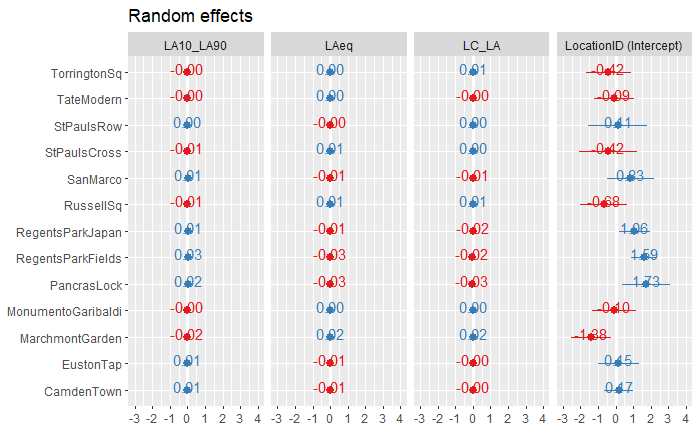
\includegraphics{Figure7.jpg}

}

\caption{\label{fig-unsclRandom}(Color online) The unscaled
location-level coefficients for the ISOPleasant model.}

\end{figure}%


\renewcommand\refname{References}
  \bibliography{../../../FellowshipRefs.bib,../FellowshipRefs.bib}


\end{document}
